\documentclass[UTF8,AutoFakeBold,AutoFakeSlant,zihao=-4]{ctexart}

\newcommand{\emp}{\noindent\fboxsep=0pt}

\usepackage{wrapfig}
\usepackage{fontspec}
\usepackage{color}
\usepackage{fancyhdr}
\usepackage{setspace}
\usepackage{caption}
\usepackage{mathptmx}
\usepackage{amsmath}
\usepackage{amssymb}
\usepackage{amstext}
\usepackage{geometry}
\usepackage{graphicx}
\usepackage{enumerate}
\usepackage{enumitem}
\usepackage{pifont}
\usepackage{float}
\usepackage{newclude}
\usepackage{subfig}
\usepackage{multirow}
\usepackage{tabularx}
\geometry{
a4paper,
left=2.5cm,
right=2.5cm,
top=2.5cm,
bottom=2.5cm,
}
%\usepackage{listings}
%\usepackage{boxedminipage}

% 设置n倍行距(需要注释掉正文中设置行距的部分)
% \linespread{1.5} % 正文1.5倍行距

%定义一级二级三级标题
\ctexset{
	section = {	% 定义一级标题 
	           	format+ = \zihao{4} \heiti \raggedright, 	% 字号为’四号‘,字体为’黑体‘,左对齐
	           	name = {,、},                             	% 序号后面加’、‘
	           	number = \chinese{section},              	% 序号为’汉字‘
	           	beforeskip = 1.0ex plus 0.2ex minus .2ex,	% 标题前的垂直间距 = 基础高度为1.0ex,可以伸展到 1.0 - 0.2 = 1.2ex,也可以收缩到 1.0 - .2 = 0.8ex; ex为当前字号下字母x的高度
	           	afterskip = 1.0ex plus 0.2ex minus .2ex, 	% 标题后的垂直间距 = ...	
	           	aftername = \hspace{0pt}                 	% 编号和标题之间的格式 = 增加水平间距’0pt‘ 
	},
	subsection = {	% 定义二级标题
	              	format+ = \zihao{-4} \songti \raggedright,
	              	name = {(,)},
	              	number = \chinese{subsection},	% 序号为’阿拉伯数字‘
	              	beforeskip = 1.0ex plus 0.2ex minus .2ex,
	              	afterskip = 1.0ex plus 0.2ex minus .2ex,
	              	aftername = \hspace{0pt},
	},
	subsubsection = {
			format+ = \zihao{-4} \songti \raggedright,
			name = {\qquad,\ \enspace},
			number = {\arabic{section}.\arabic{subsection}.\arabic{subsubsection}},	
			beforeskip = 1.0ex plus 0.2ex minus .2ex,
			afterskip = 1.0ex plus 0.2ex minus .2ex,
			aftername = \hspace{0pt},
	}
}

% 设置页眉页码
\pagestyle{plain} % 取消页眉
\lfoot{}	% 页码出现在下方

% 定义正文字体
\setromanfont{Times New Roman}	% 将西文字体设置为 Times New Roman
% \setCJKfamilyfont{zhkai}{[SIMKAI.TTF]}
% \newcommand*{\kaiti}{\CJKfamily{zhkai}}

% 定义 caption
\DeclareCaptionFont{kaiticaption}{\kaishu \small}	% 定义下面三个caption的font的kaiticaption的具体格式
\captionsetup[figure]{font=small,labelsep=quad,skip=0.5ex,labelfont=bf,font=kaiticaption}	% 设置图片的 caption 格式 % 想要标题换行后居中,可以添加justification=centering
\captionsetup[table]{font=small,labelsep=quad,skip=0.5ex,labelfont=bf,font=kaiticaption}	% 设置表格的 caption 格式
\captionsetup[subfloat]{font=small,labelsep=quad,skip=0.5ex,labelfont=bf,font=kaiticaption}
\captionsetup[equation]{font=small,labelsep=quad,skip=0.5ex,labelfont=bf,font=kaiticaption}


% 设置图片,表格,公式编号格式
\renewcommand{\thetable}{\thesection{}-\arabic{table}}	% \thetable 表示设置的是表格的编号格式, 后面括号的内容为编号格式:章节号-表格的序号
\renewcommand{\thefigure}{\thesection{}-\arabic{figure}}
\renewcommand{\theequation}{\thesection{}-\arabic{equation}}

% 设置列表标签
\setlist[enumerate]{nosep,itemindent=0.75em,labelsep=0.5em}	% labelsep 是标签与标签后面内容的间距(这里是一个空格),leftmargin是标签后面内容与左边界之间的距离
\setlist[itemize]{nosep,itemindent=0.5em, labelsep=0.5em}
\setlist[description]{nosep,leftmargin=*}
\let\olddescriptionlabel\descriptionlabel  
\renewcommand{\descriptionlabel}[1]{\hspace{2em}\olddescriptionlabel{#1}:}  


% 设置代码块
%\definecolor{commentcolor}{RGB}{85,139,78}
%\definecolor{stringcolor}{RGB}{206,145,108}
%\definecolor{keywordcolor}{RGB}{34,34,250}
%\lstset{
%	language=Matlab, % 默认代码语言.
%	basicstyle=\footnotesize,
%	numbers=left, %设置行号位置
%	numberstyle=\tiny, %设置行号大小
%	commentstyle=\color{commentcolor},	%注释颜色
%	keywordstyle=\color{keywordcolor},	%关键词颜色
%	stringstyle=\color{stringcolor},	%字符串颜色
%	frame=single, %设置边框格式
%	escapeinside=``, %逃逸字符(1左面的键),用于显示中文
%	breaklines = True, % 自动折行
%	breakatwhitespace = True, % 自动折行时打断单词
%	extendedchars=false, %解决代码跨页时,章节标题,页眉等汉字不显示的问题
%	xleftmargin=2em,xrightmargin=2em, aboveskip=1em, %设置边距
%	tabsize=4, %设置tab空格数
%	showspaces=false %不显示空格
%}

\graphicspath{{../img/}}
\title{底盘系统}
\author{}
\date{}
\usepackage{extarrows}
\begin{document}
\setlength{\parskip}{0em}	% 段前段后间距为 0
\setlength{\parindent}{2em} % 正文首行悬挂: 2汉字字符
\setlength{\baselineskip}{20pt}	% 正文行间距20磅
\selectfont	% 刷新行间距信息
\setlength{\lineskip}{10pt}		% 推荐设置为行距的一半
\setlength{\lineskiplimit}{10pt}	% 同上
\abovedisplayshortskip=0pt	%设置公式距离上方非重叠区域额外添加的距离,推荐0
\belowdisplayshortskip=0pt
\abovedisplayskip=0pt	%设置公式距离上方重叠距离额外添加的距离,推荐0
\belowdisplayskip=0pt
\renewcommand{\arraystretch}{1.5}
\maketitle

\section{overview}
	\vspace{-1.8em}
	\begin{wrapfigure}{R}{0cm}
		\centering
		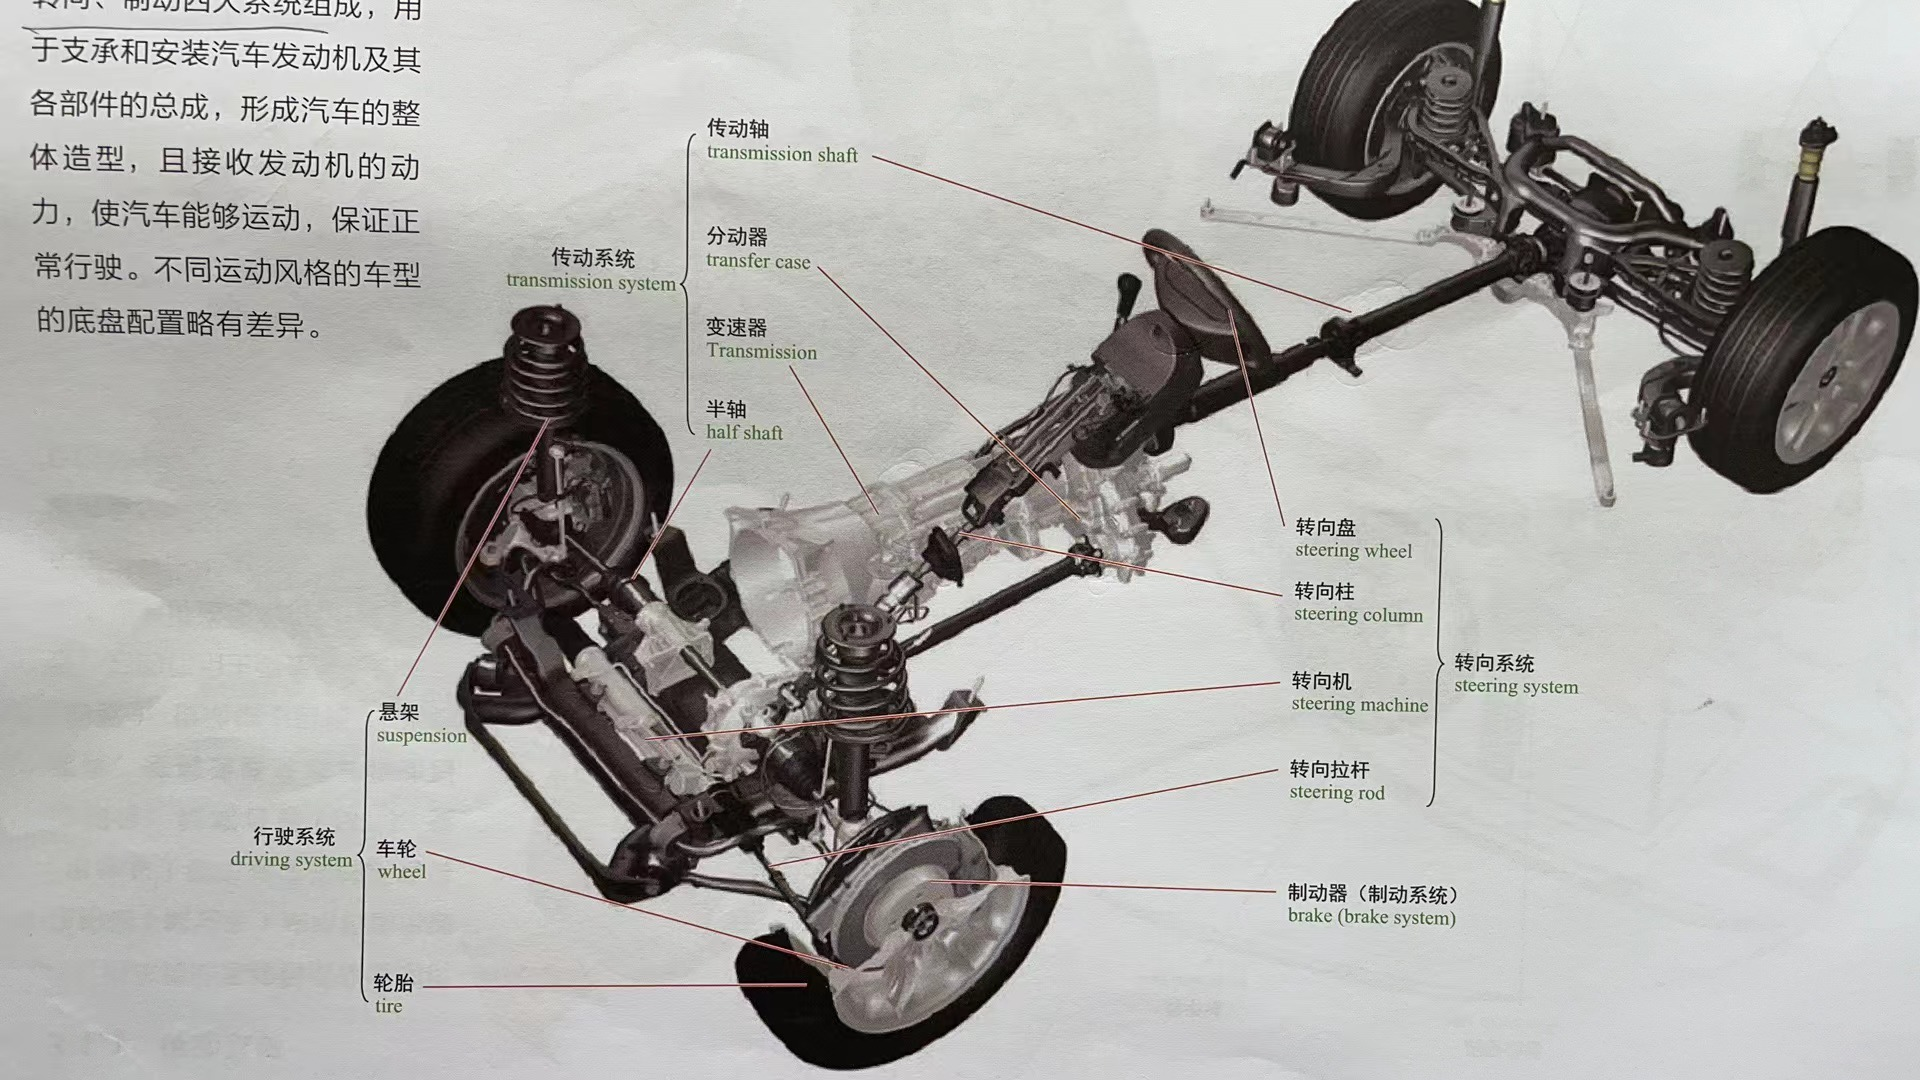
\includegraphics[width=0.7\textwidth]{3-1}
	\end{wrapfigure}
	\begin{equation*}
		\text{底盘系统}\begin{cases}
			\text{传动系统} \\
			\text{行驶系统} \\
			\text{转向系统} \\
			\text{制动系统}
		\end{cases}
	\end{equation*}
\vspace{6em}
\subsection{传动系统}
	\begin{itemize}
		\item 作用:传递发动机输出的动力 to 车辆
		\item components:
		\[ \underset{\text{燃油车}}{\text{发动机飞轮端}} \underset{components}{\longleftrightarrow} wheel \longleftrightarrow \underset{\text{电车}}{\text{电机的输出轴}} \]
	\end{itemize}
	\begin{center}
		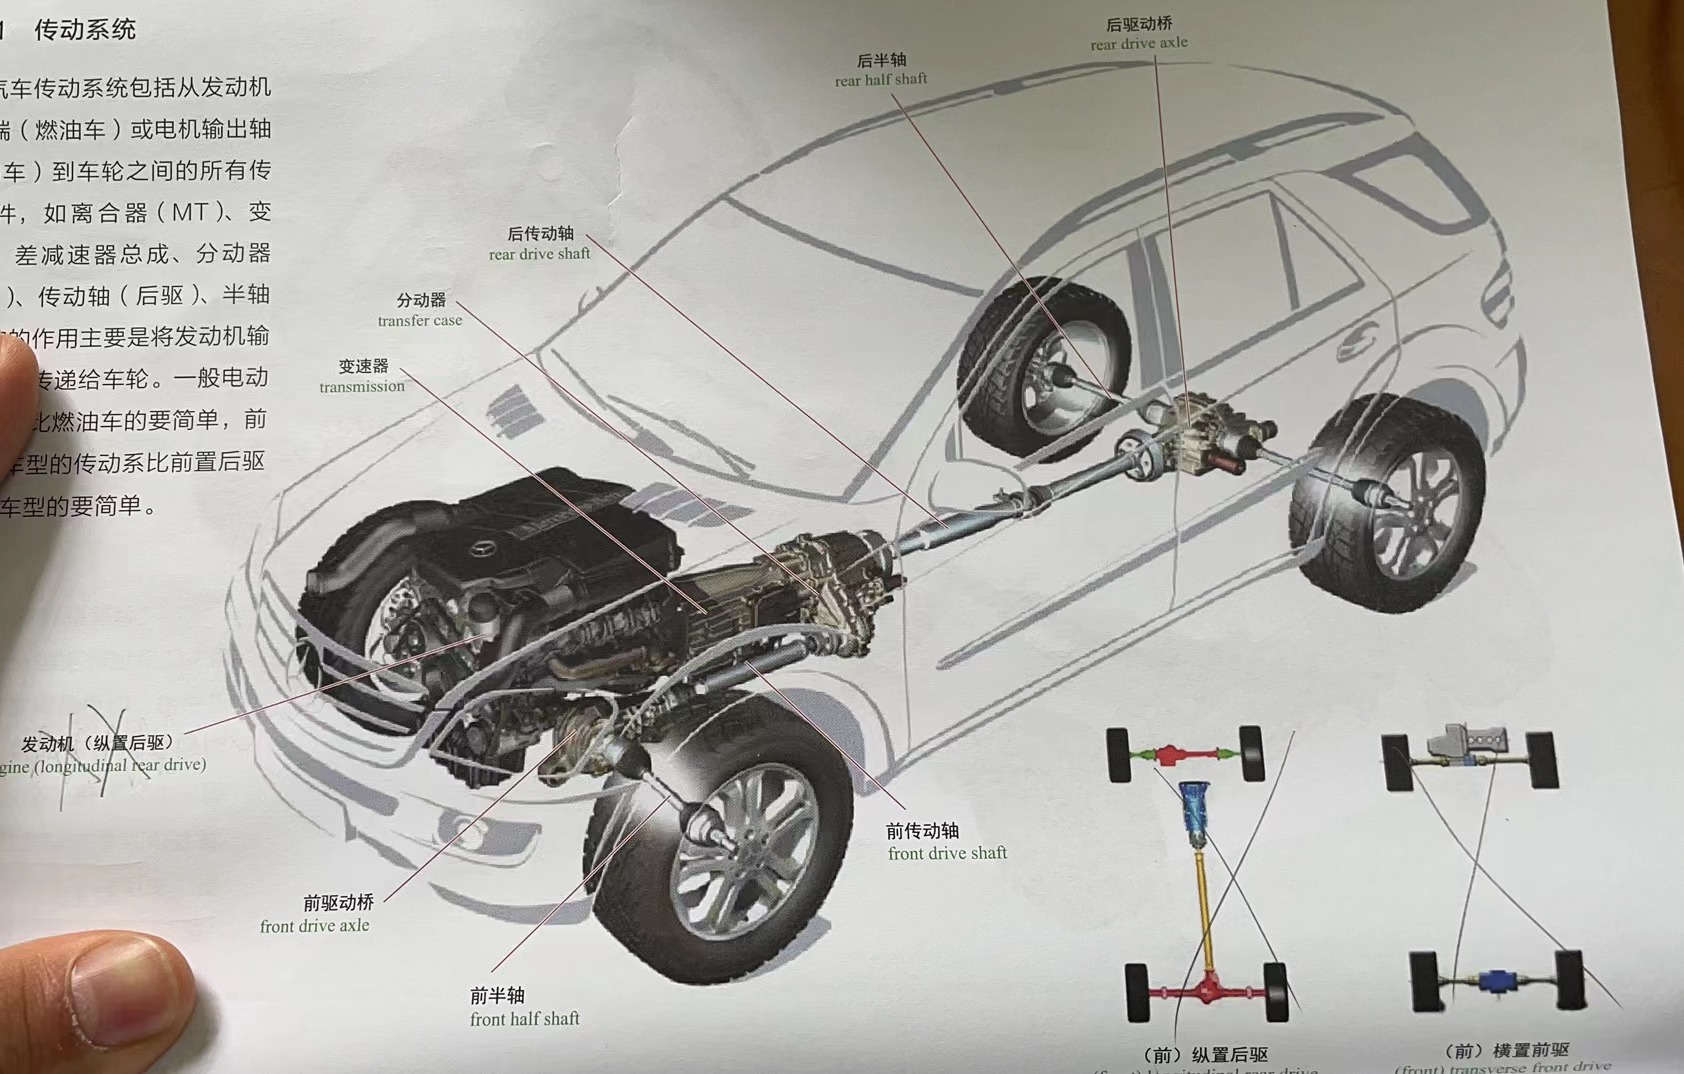
\includegraphics[width=0.6\linewidth]{3-2}
	\end{center}
\subsection{行驶系统}
	\begin{itemize}
		\item function: 将汽车构成一个整体
		\item components:
		$\begin{cases}
			\parbox{.8\linewidth}{车架(汽车一般是承载式车身,集成了车架;卡车一般是非承载式车身,车架不整合到车身中):一般是有两根纵梁和几根横梁组成的架子} \\
			\text{副车架(承载式车身):支撑前/后桥和悬挂的支架} \\
			\text{悬架(悬架)} \\
			\text{车桥} \\
			\text{轮胎}
		\end{cases} $
	\end{itemize}
	\begin{center}
		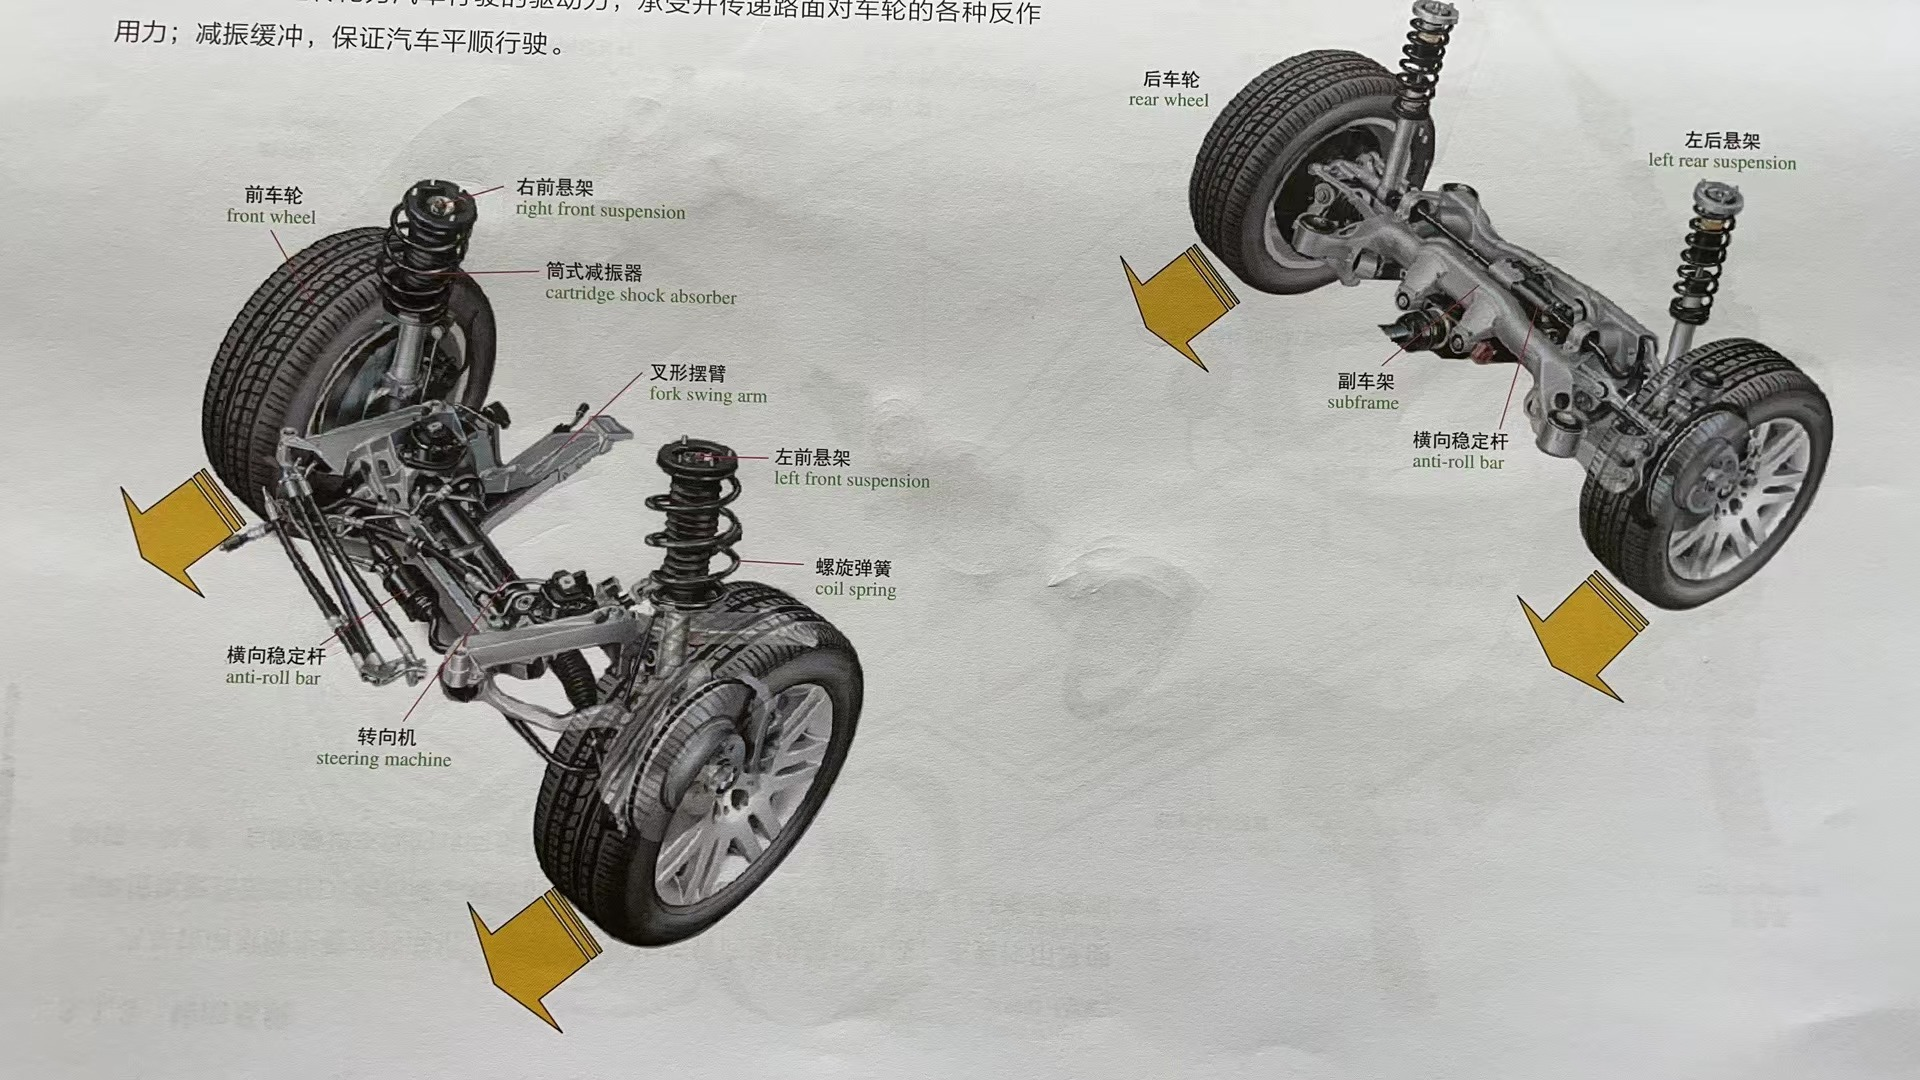
\includegraphics[width=.8\textwidth]{3-3}
	\end{center}
\subsection{转向系统}
	\begin{itemize}
		\item components
			$ \begin{cases}
				\text{转向机} \\
				\text{转向传动机构} \\
				\text{转向操纵机构}
			\end{cases} $
		\item types
			$ \begin{cases}
				\text{EPS(electric power steering system) 电动助力转向系统} \\
				\text{HPS(hydraulic power steering system) 液压助力转向系统}
			\end{cases} $
	\end{itemize}
	\begin{center}
		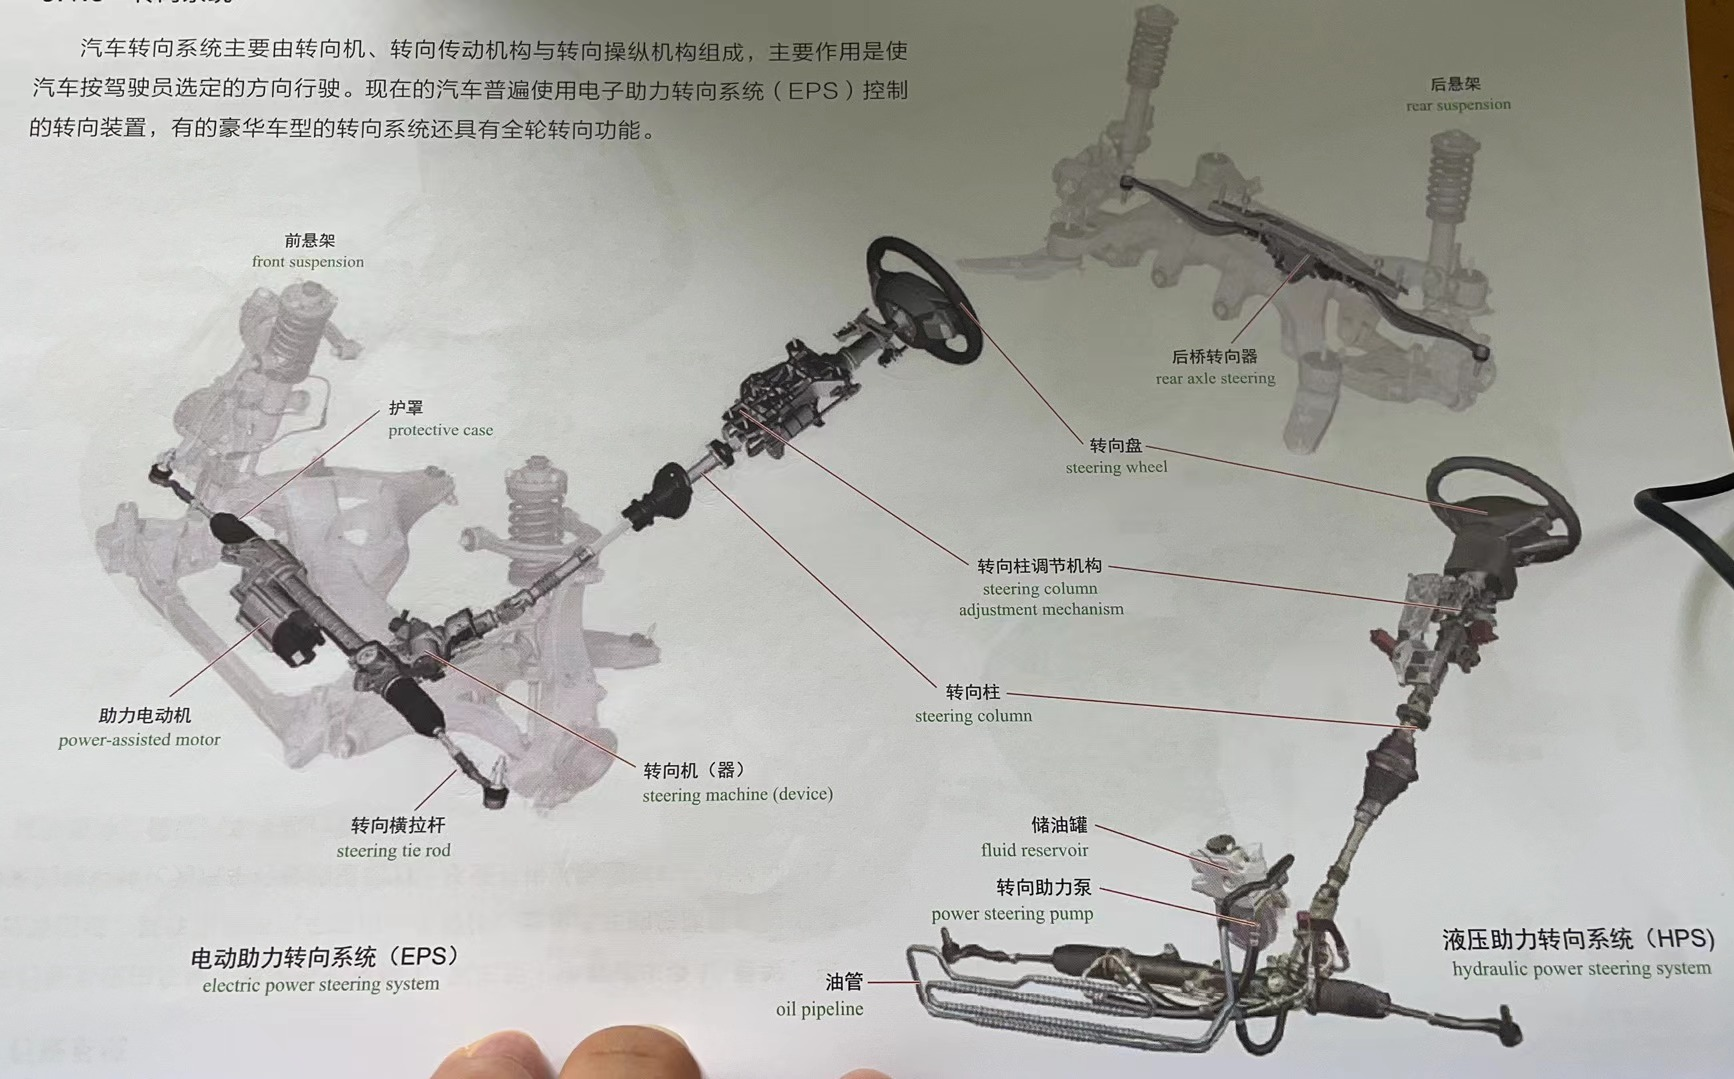
\includegraphics[width=.9\textwidth]{3-4}
	\end{center}
\subsection{制动系统}
	\subsubsection{components}
		行车制动、驻车制动
	\subsubsection{types}
		ABS(antilock brake system) 防抱死制动系统(常用)
		
		ESP(electric stability program) 稳定控制系统(高端车)
	\begin{center}
		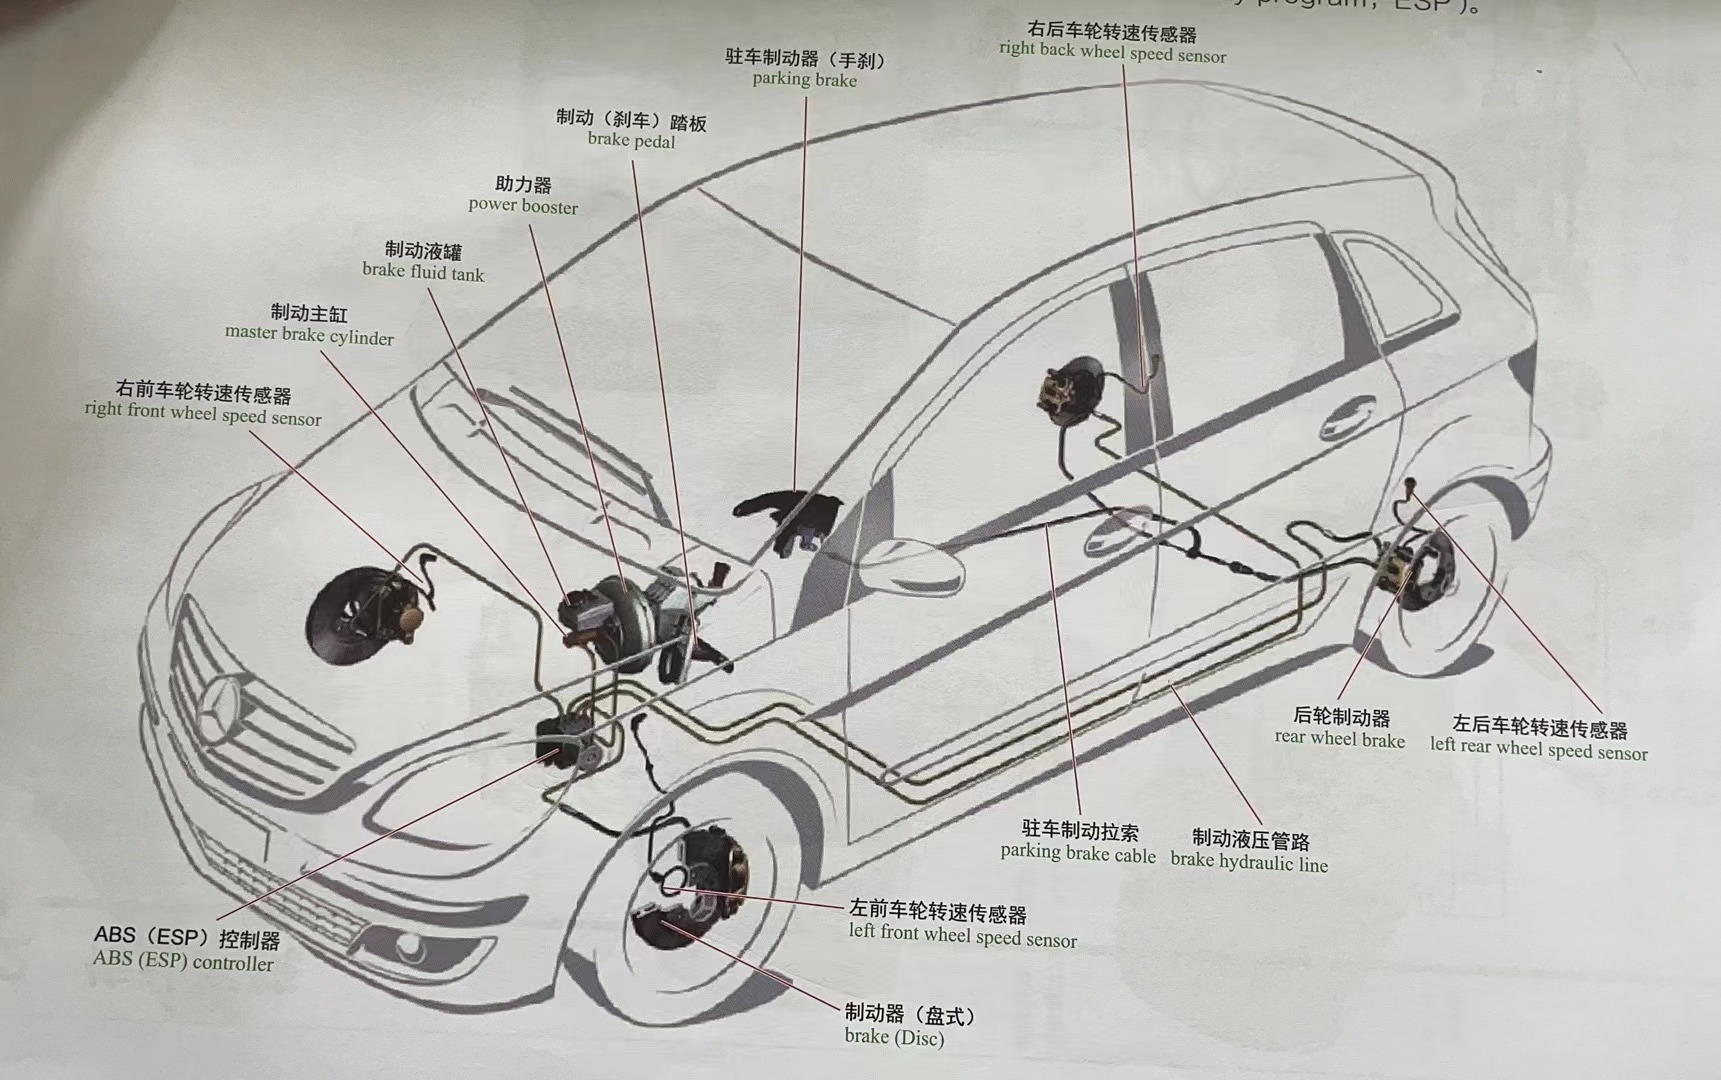
\includegraphics[width=0.6\textwidth]{3-5}
	\end{center}
\section{传动系统}
\subsection{布置形式}
	\begin{wrapfigure}{R}{0cm}
		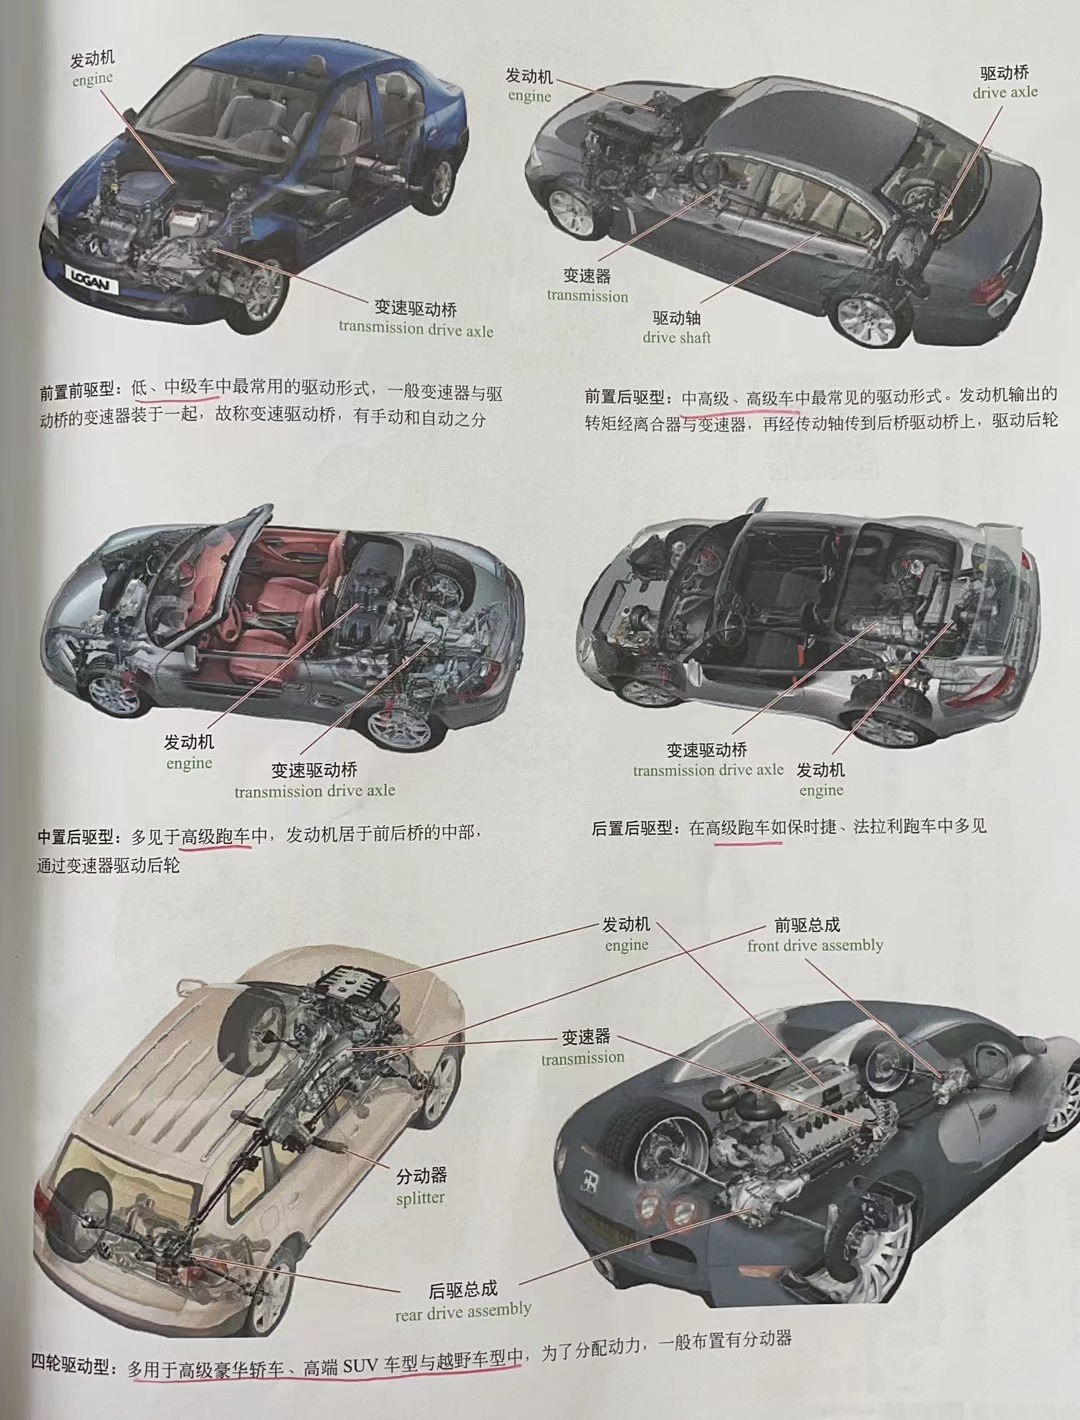
\includegraphics[width=0.7\textwidth]{3-6}
	\end{wrapfigure}
	\begin{equation*}
		\begin{cases}
			\text{FR 发动机前置后驱} \\
			\text{FF} \\
			\text{RR} \\
			\text{MR} \\
			\text{4WD 四轮驱动} \\
		\end{cases}
	\end{equation*}
\clearpage
	\subsection{五档手动变速器驱动桥}
		变速驱动桥整合了变速器、驱动桥,不包括离合器
		\begin{center}
		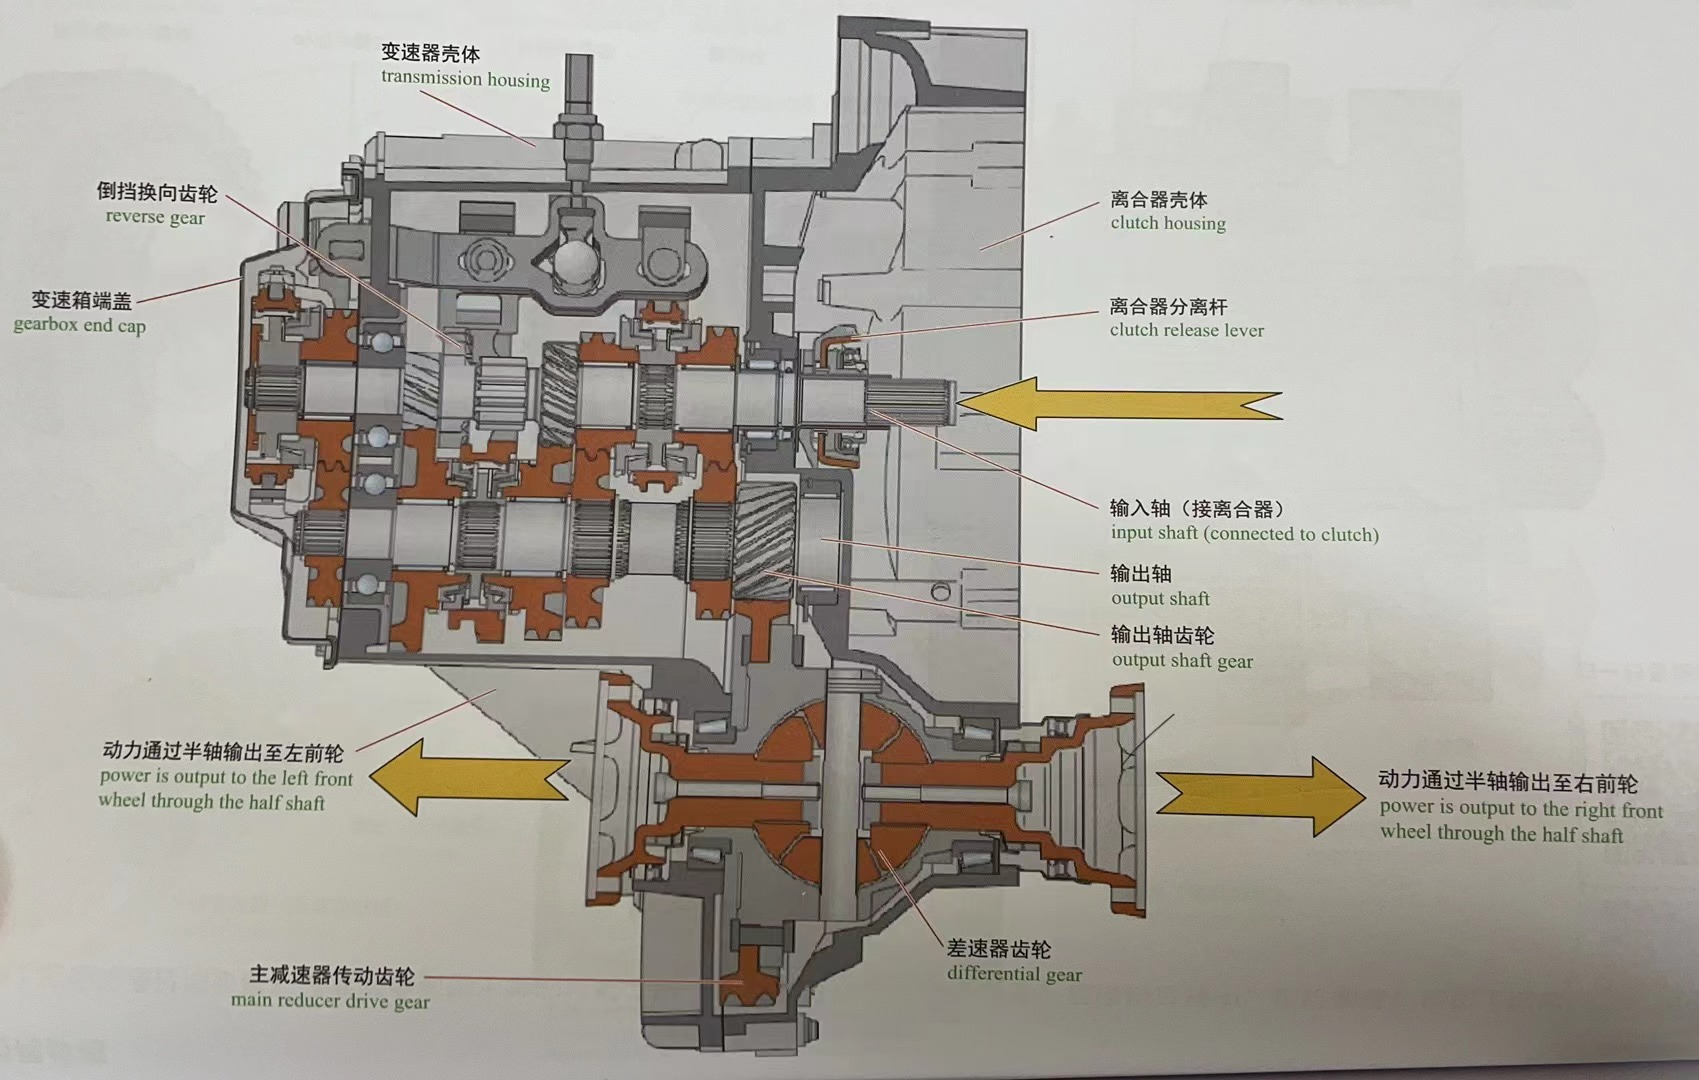
\includegraphics[width=0.5\textwidth]{3-12}
		\end{center}
	\subsection{五档手动变速器结构}
		\begin{center}
			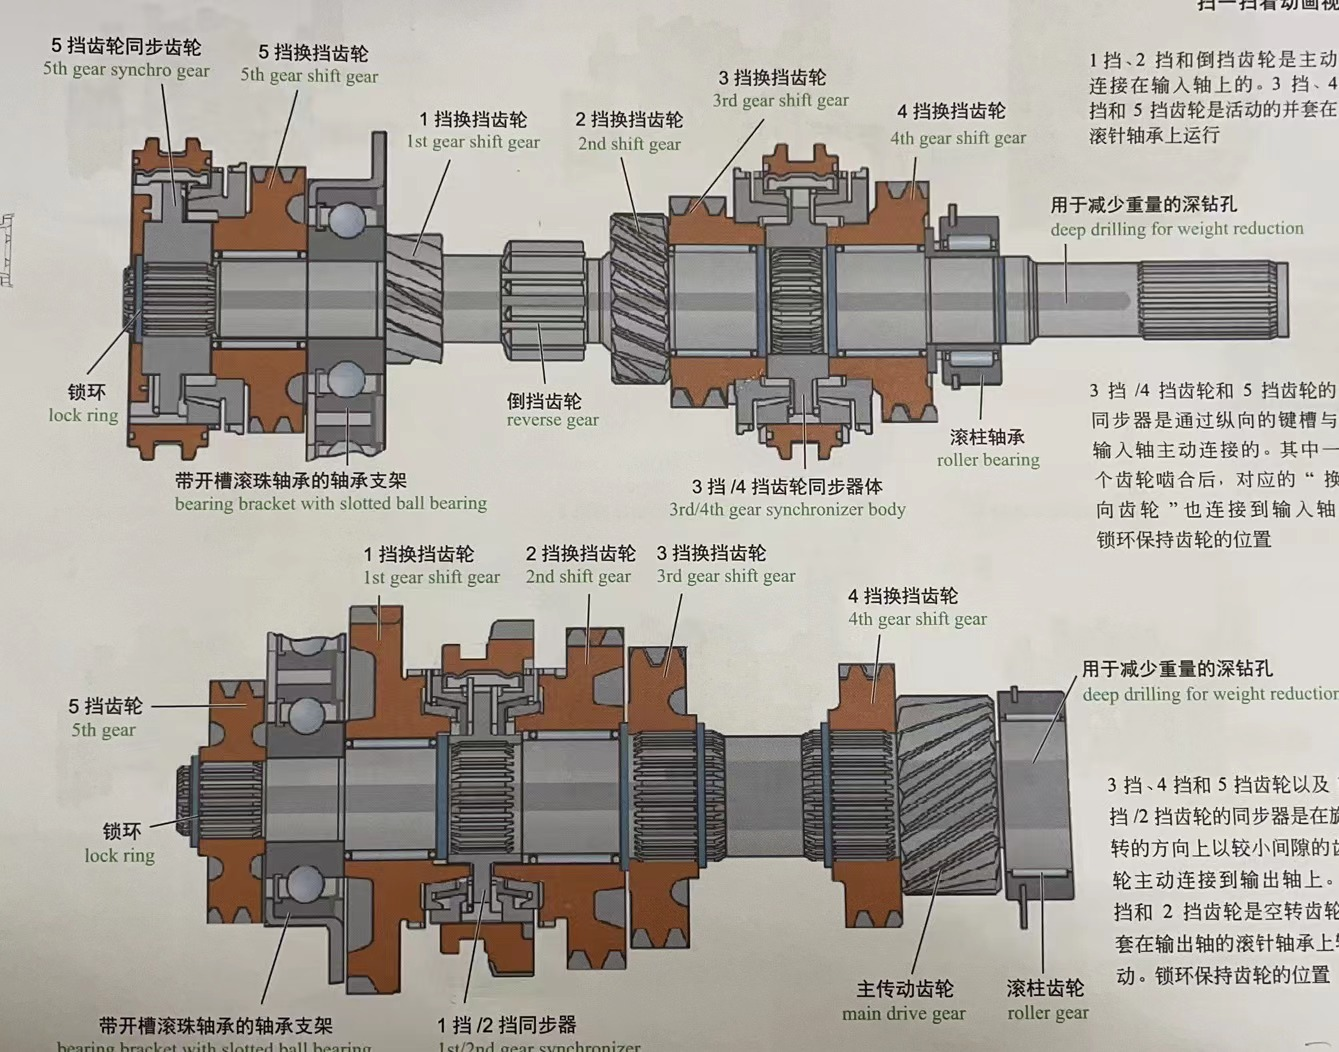
\includegraphics[width=0.5\textwidth]{3-13}
		\end{center}
	\subsection{五档手动变速器原理}
			\begin{center}
				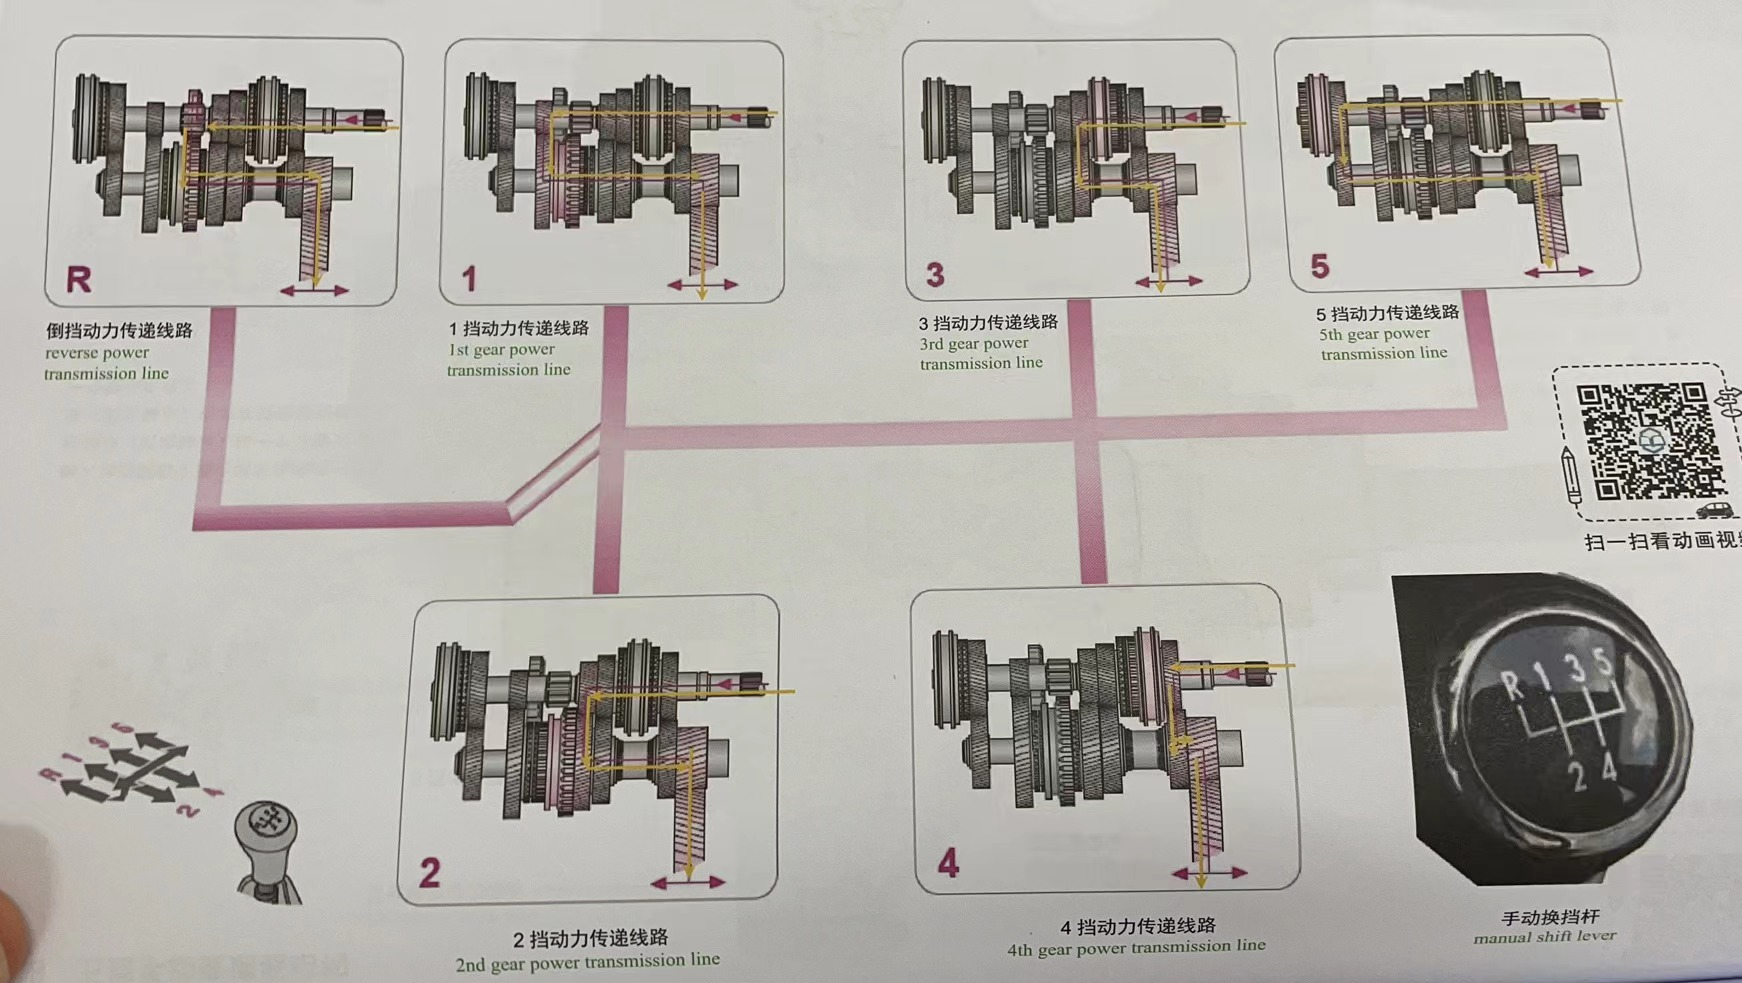
\includegraphics[width=0.5\textwidth]{3-14}
			\end{center}
	\subsection{自动变速器结构(常规)}
		档位一般位倒档R、空档N、前进档D、驻车档P、手动档M/S
		\begin{center}
			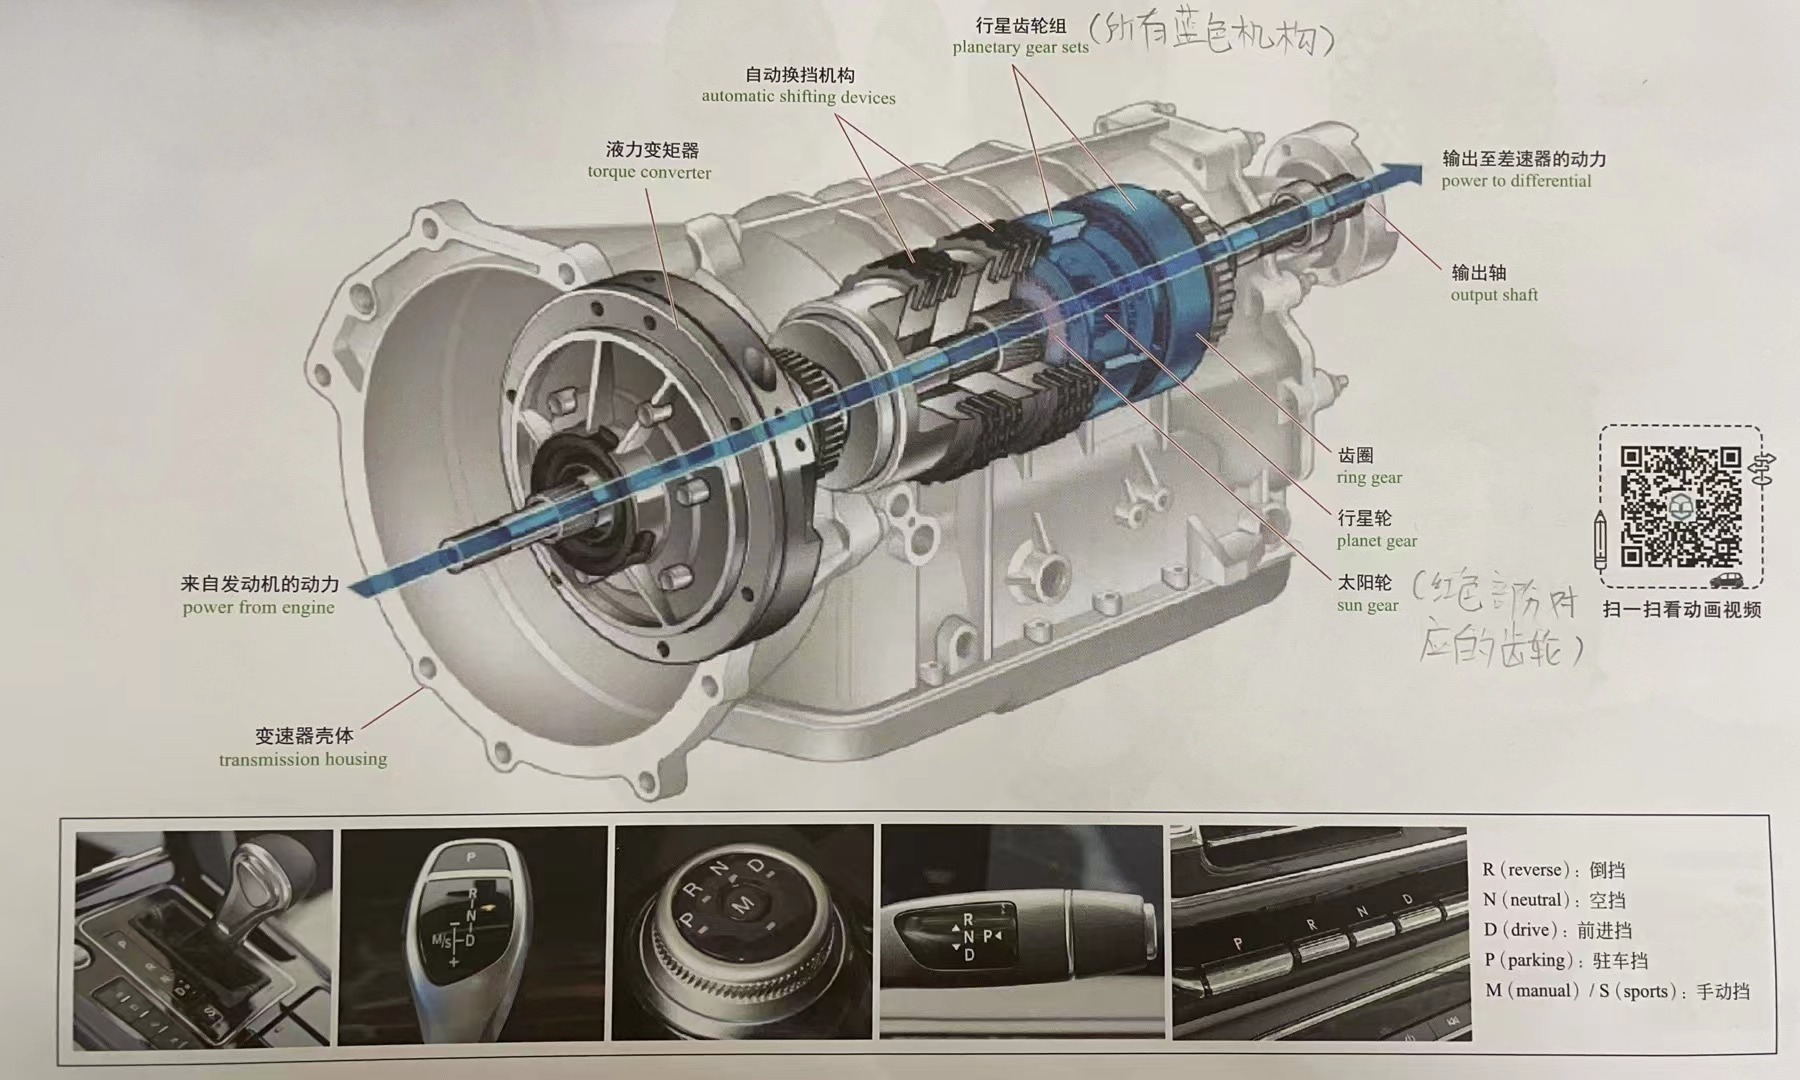
\includegraphics[width=0.5\textwidth]{3-15}
		\end{center}
	\subsection{液力变矩器}
		\begin{center}
			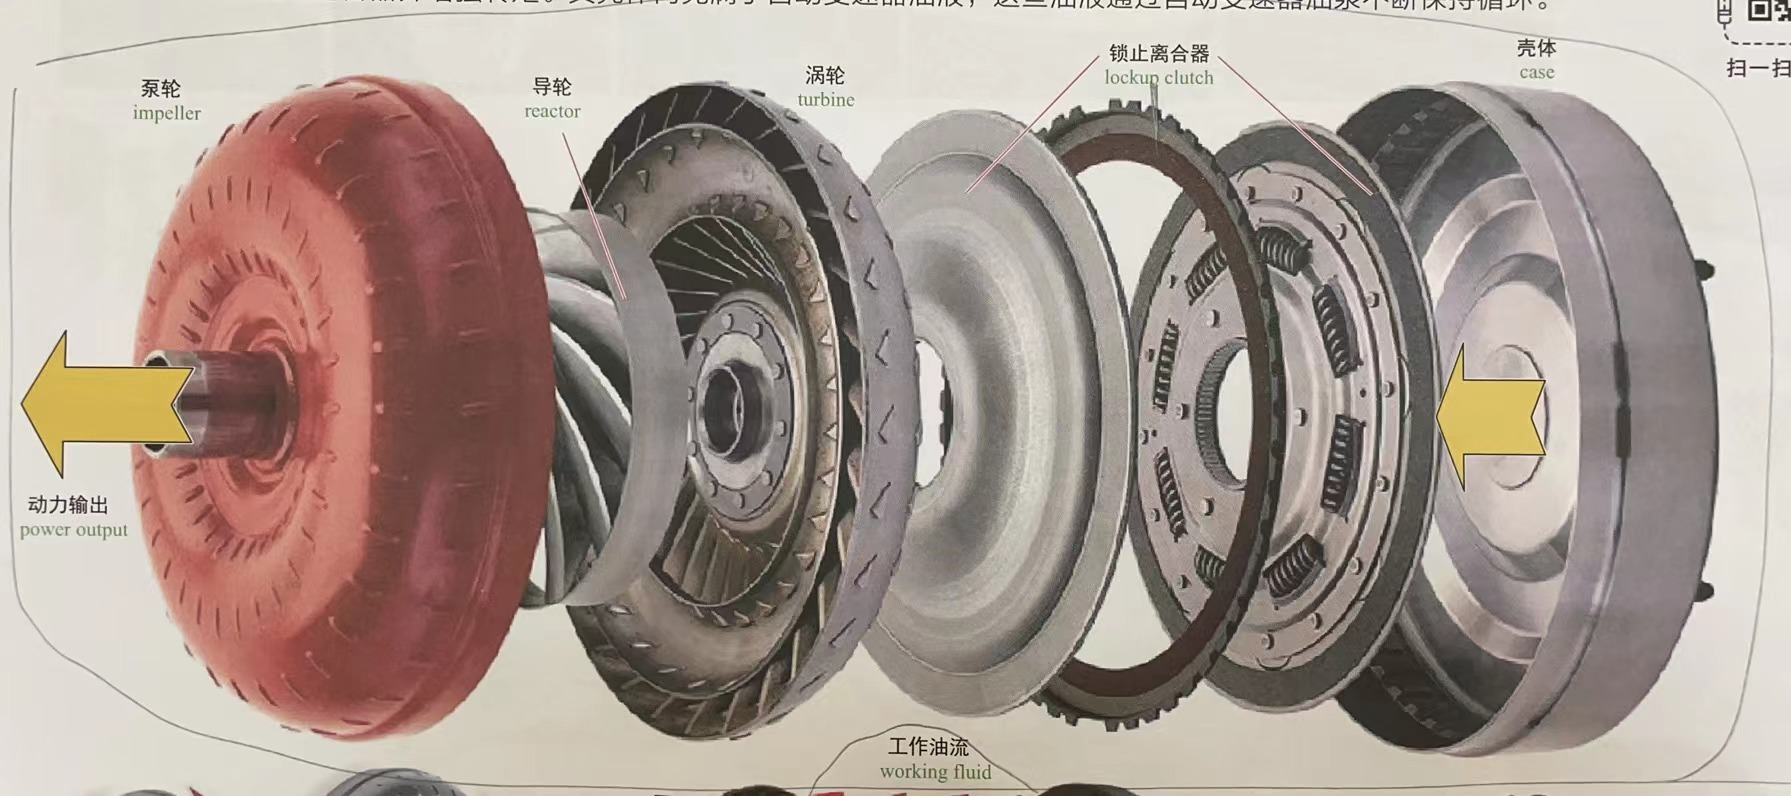
\includegraphics[width=0.5\textwidth]{3-16}
		\end{center}
		\begin{enumerate}[label*=\arabic*)]
			\item 自动挡汽车一般没有单独的离合器,靠自动变速器内的液力变矩器提供离合器的功能
			\item 将发动机转矩传送到行星齿轮组
		\end{enumerate}
	\subsection{行星齿轮组}
		\begin{center}
			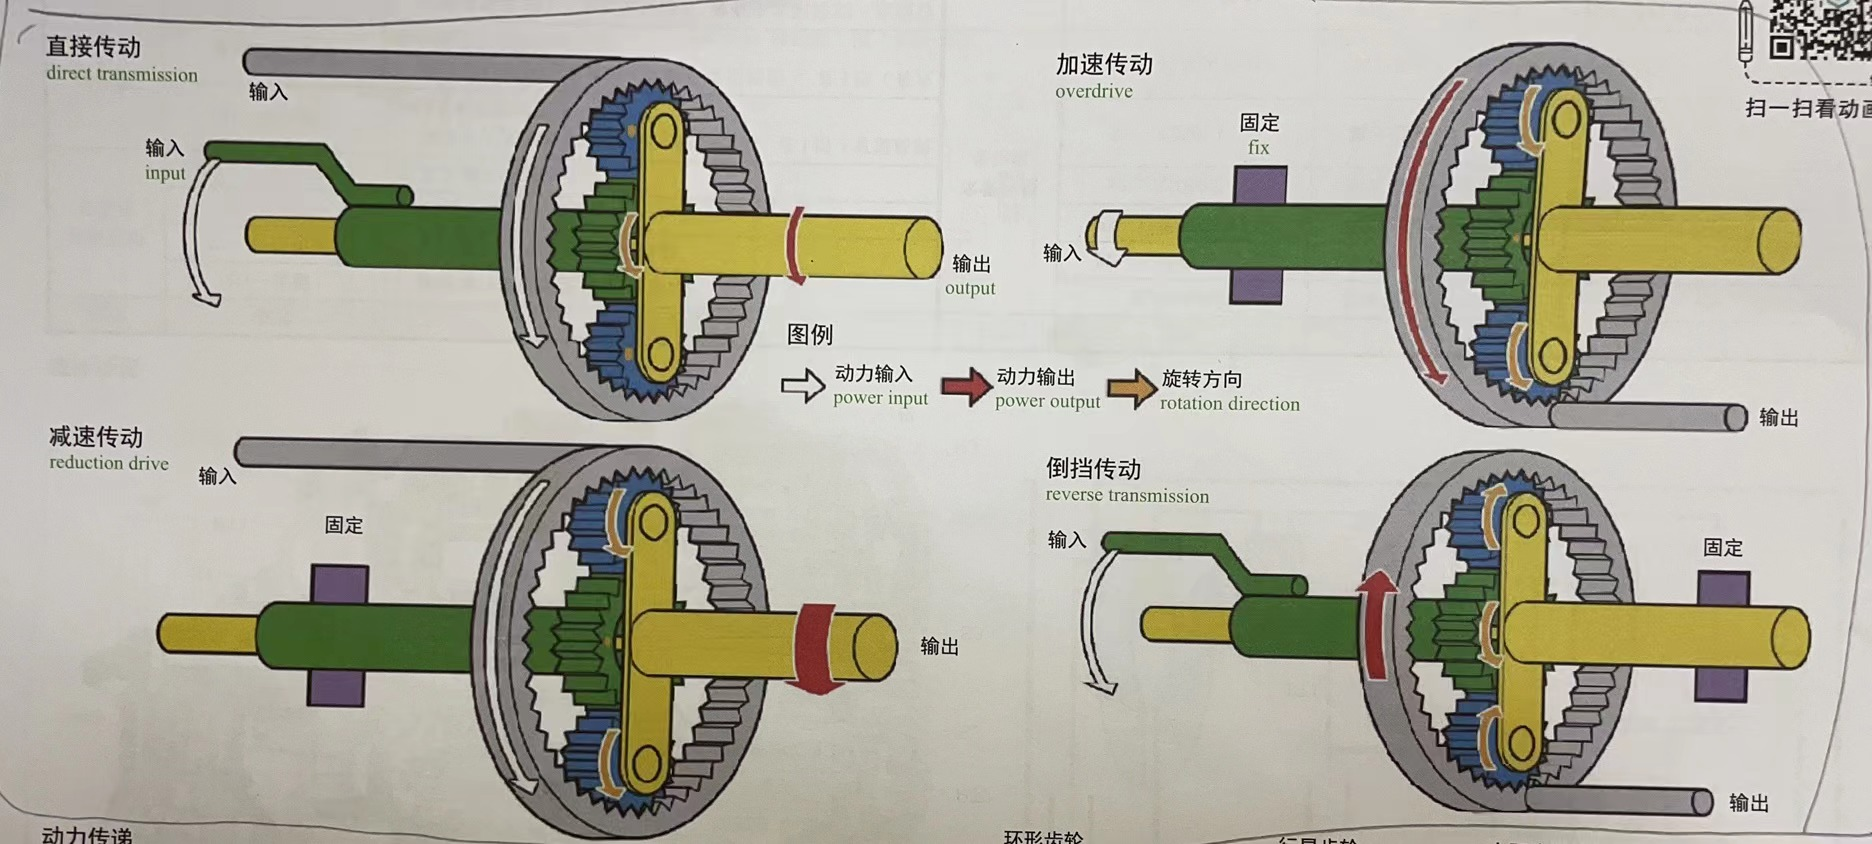
\includegraphics[width=0.5\textwidth]{3-17}
		\end{center}
	\subsection{六档自动变速器}
		\begin{center}
			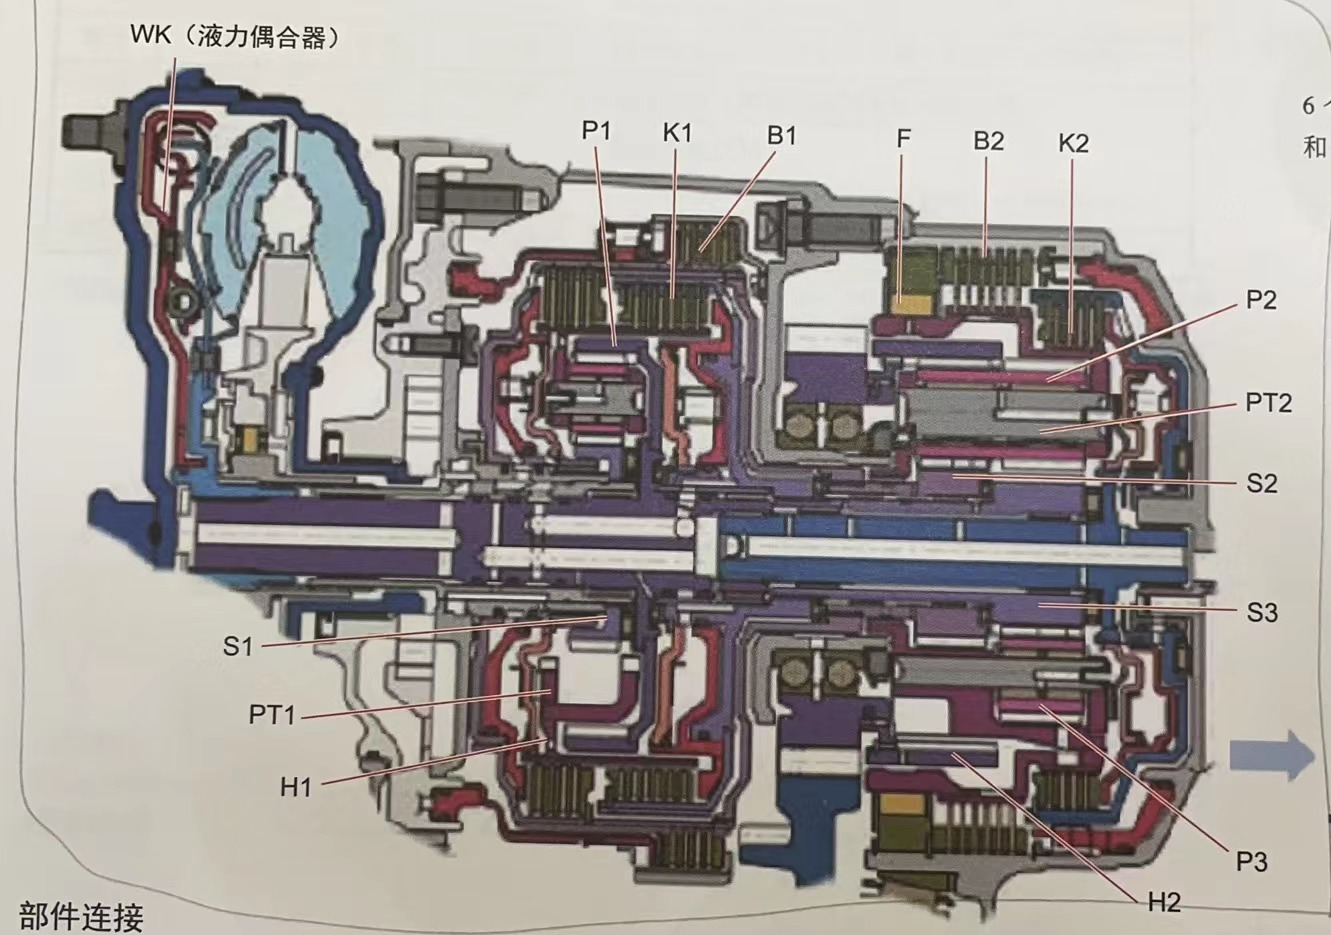
\includegraphics[width=0.5\textwidth]{3-18}
			
			集成了2个离合器、制动器、初级行星齿轮组、次级行星齿轮组
		\end{center}
	\subsection{双离合变速器}
		\begin{enumerate}
			\item 介绍
				
				双离合变速器建成DCT(dual cluctch transmission),又称DSG(direct shaft gearbox),有两个离合器$ \begin{cases}
					\text{一个对应奇数档,一个对应偶数档} \\
					\text{不能同时接合}
				\end{cases} $
			
				档车辆挂入一个档位,只要当前档位分离即可立即接入下一档位
				
				常规自动变速器没有数字档,双离合变速器有数字档和常规自动变速器档位
				\begin{center}
					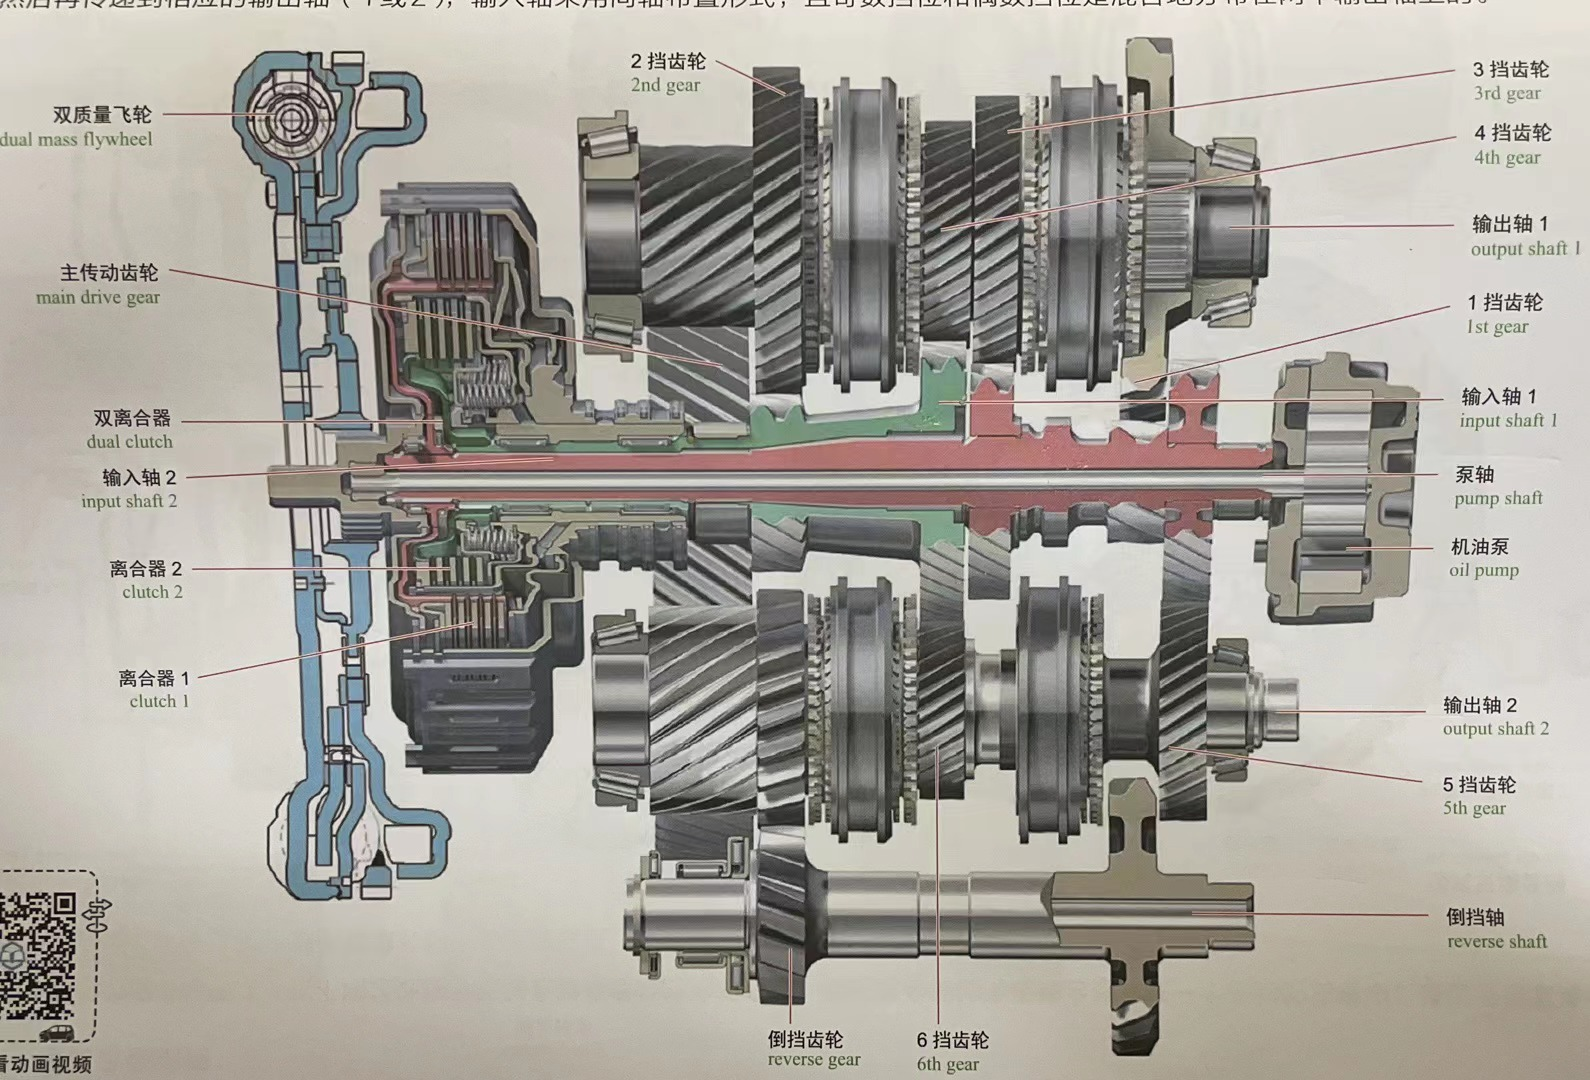
\includegraphics[width=0.5\textwidth]{3-22}
				\end{center}
			\item 种类: 干式(风冷)和湿式(油冷)
				\begin{figure}[htbp]
					\centering
					\caption{\footnotesize 湿式离合器}
					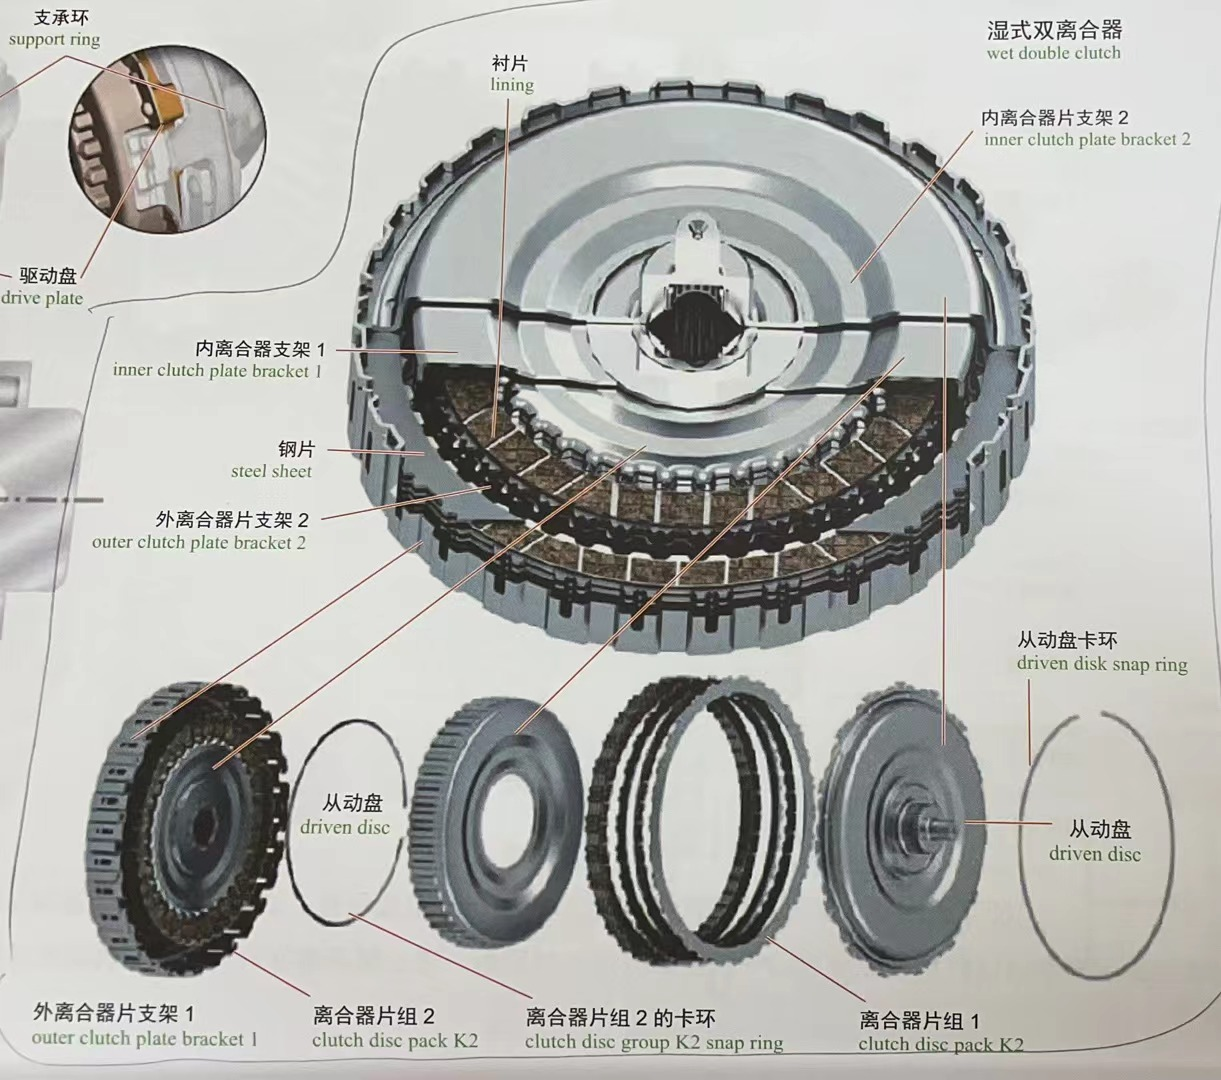
\includegraphics[width=0.5\textwidth]{3-20}
				\end{figure}
		\end{enumerate}
	\clearpage
	\subsection{七档湿式双离合变速器}
		动力传递
		\begin{center}
			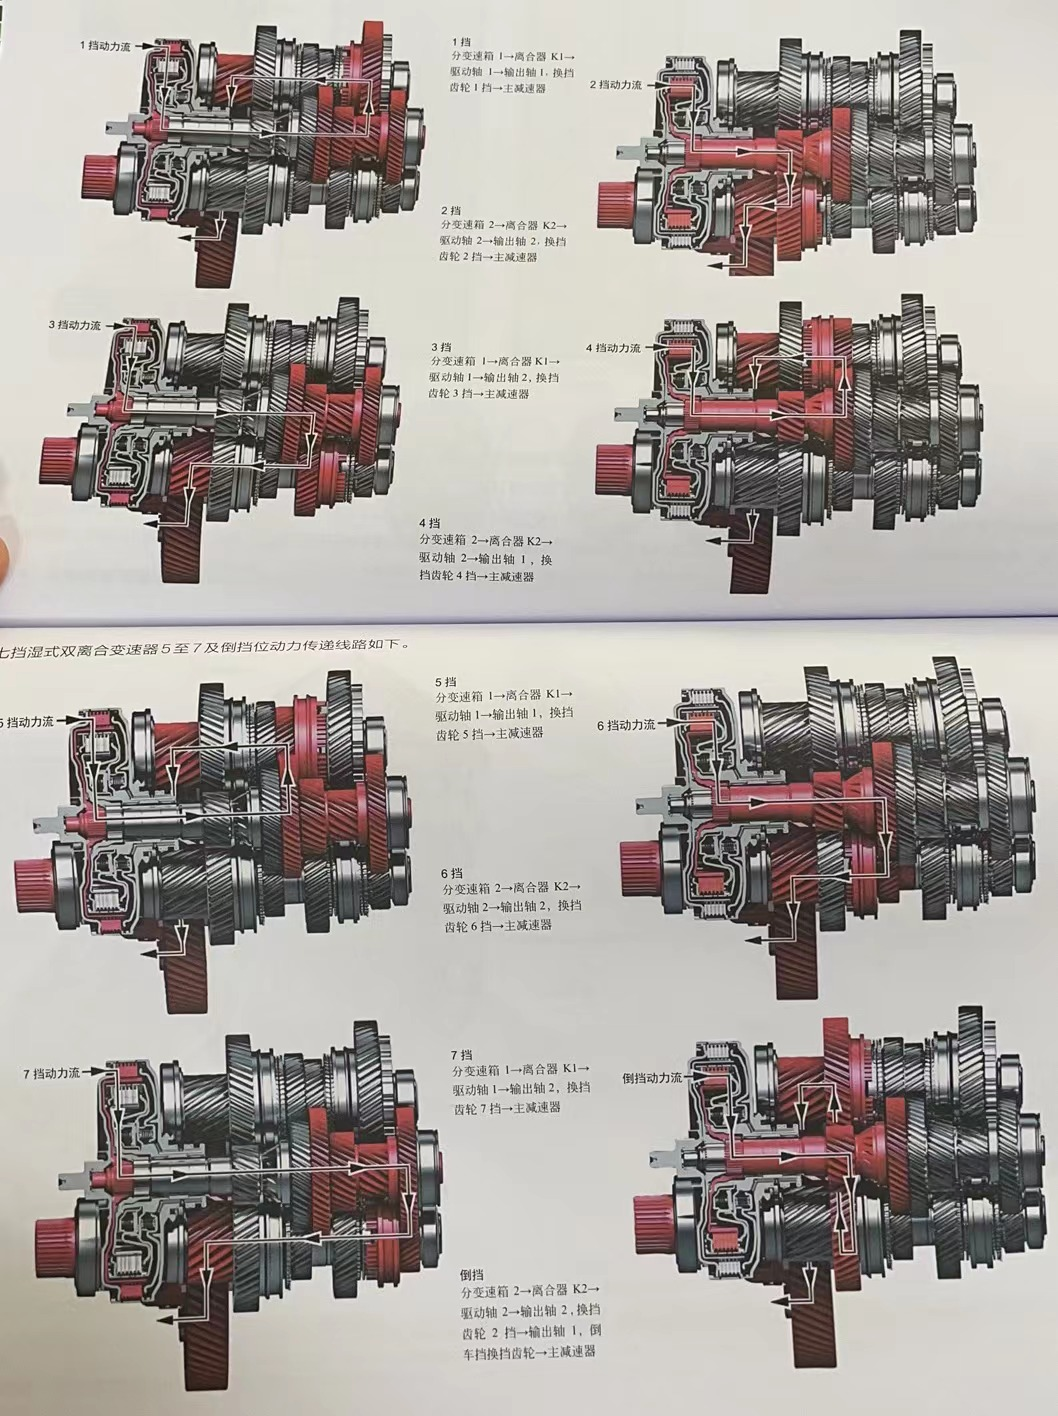
\includegraphics[width=0.5\textwidth]{3-21}
		\end{center}
	\subsection{六档湿式双离合变速器}
		\begin{center}
			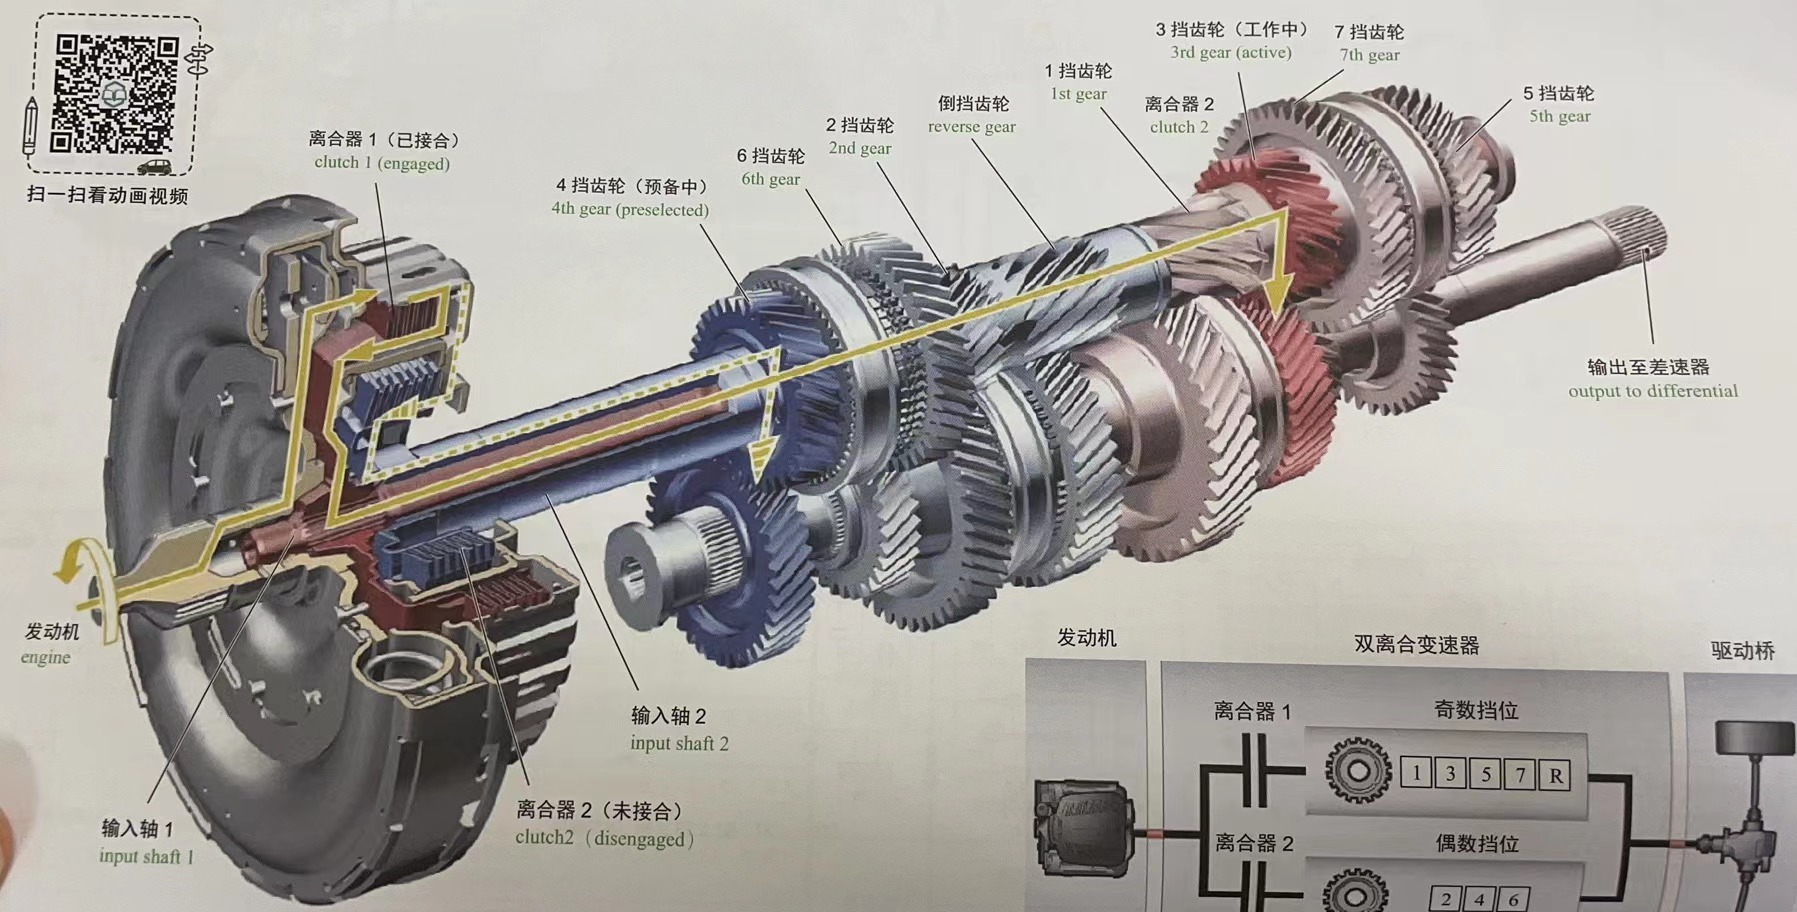
\includegraphics[width=0.5\textwidth]{3-19}
		\end{center}
	\clearpage
	\subsection{离合器}
		不包括飞轮,但一般安装在飞轮上。用于切断/传递发动机到变速器的动力
		\begin{center}
			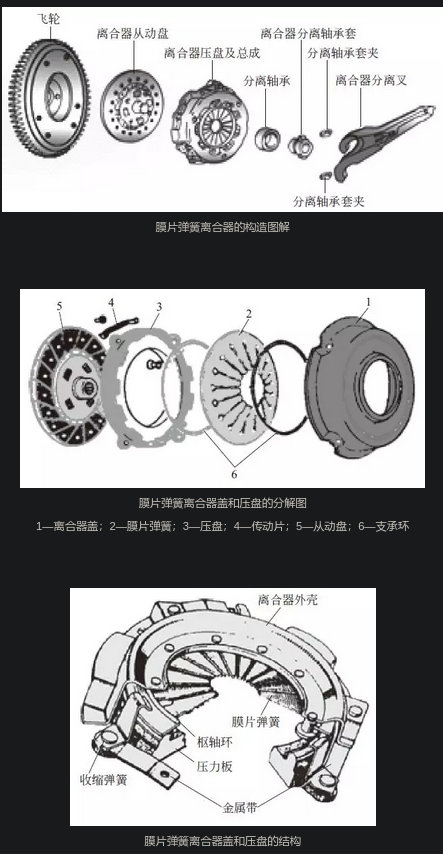
\includegraphics[width=0.5\textwidth]{3-7}
		\end{center}
	\subsection{换挡同步器}
		类似于离合器 between 变速器 and 换挡齿轮
	\subsection{无级变速器}
		属于自动变速器
		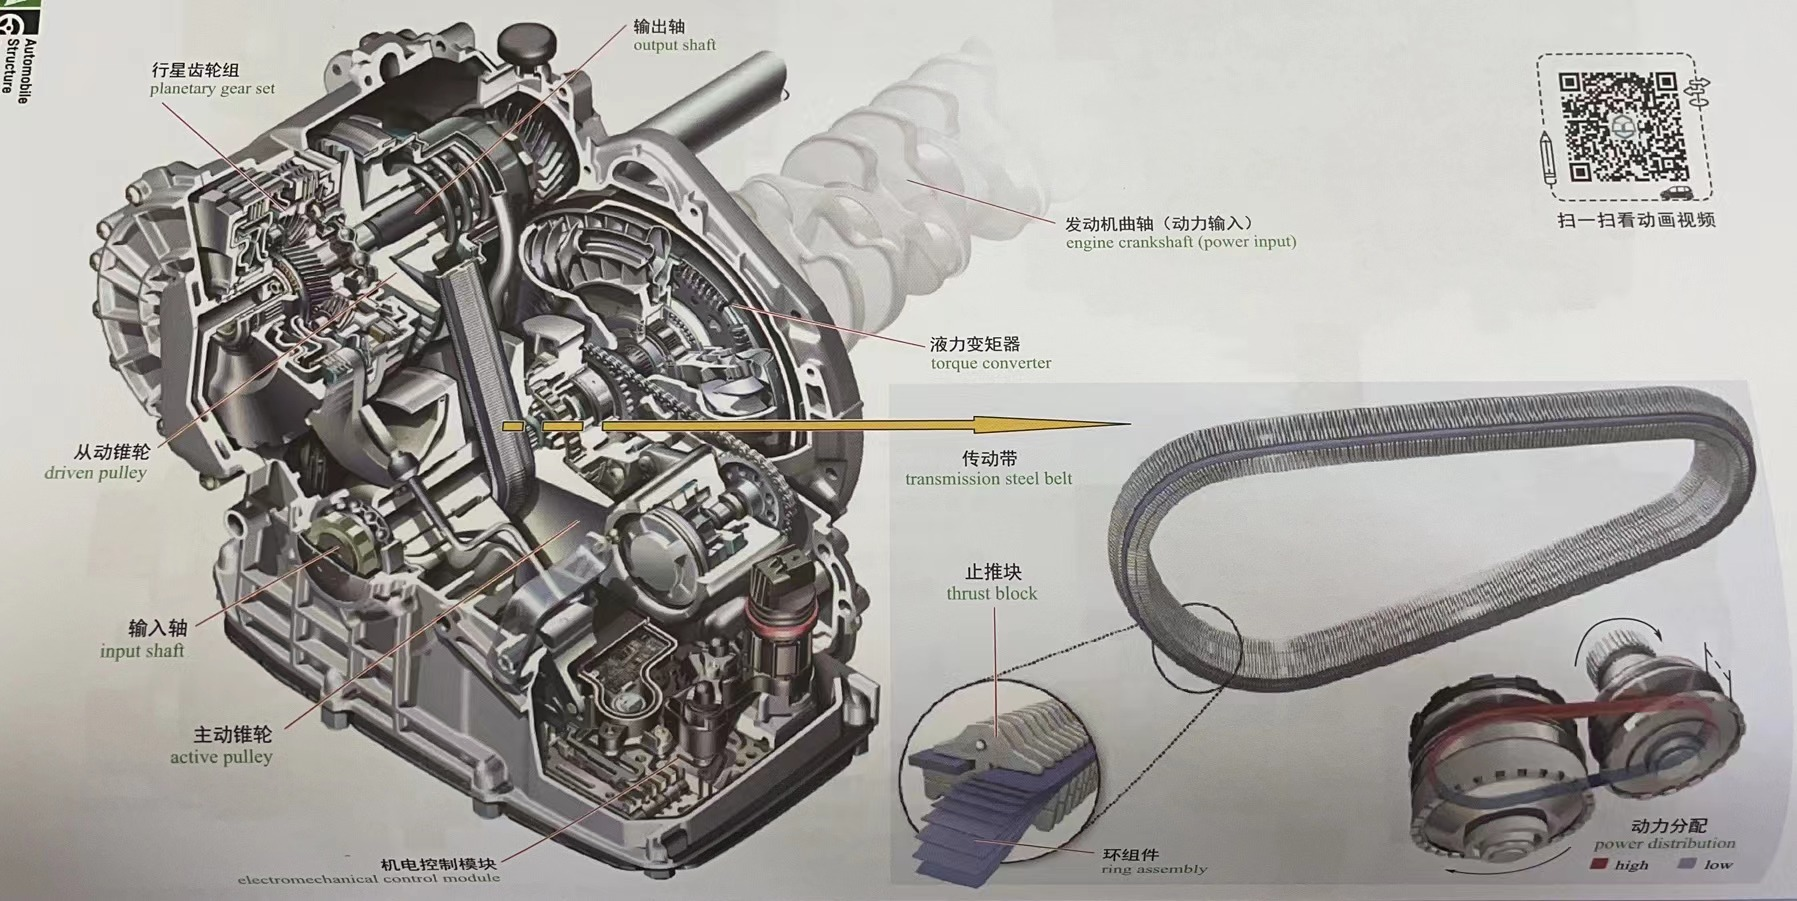
\includegraphics[width=0.5\textwidth]{3-8}
	\subsection{四轮驱动4WD/AWD}
		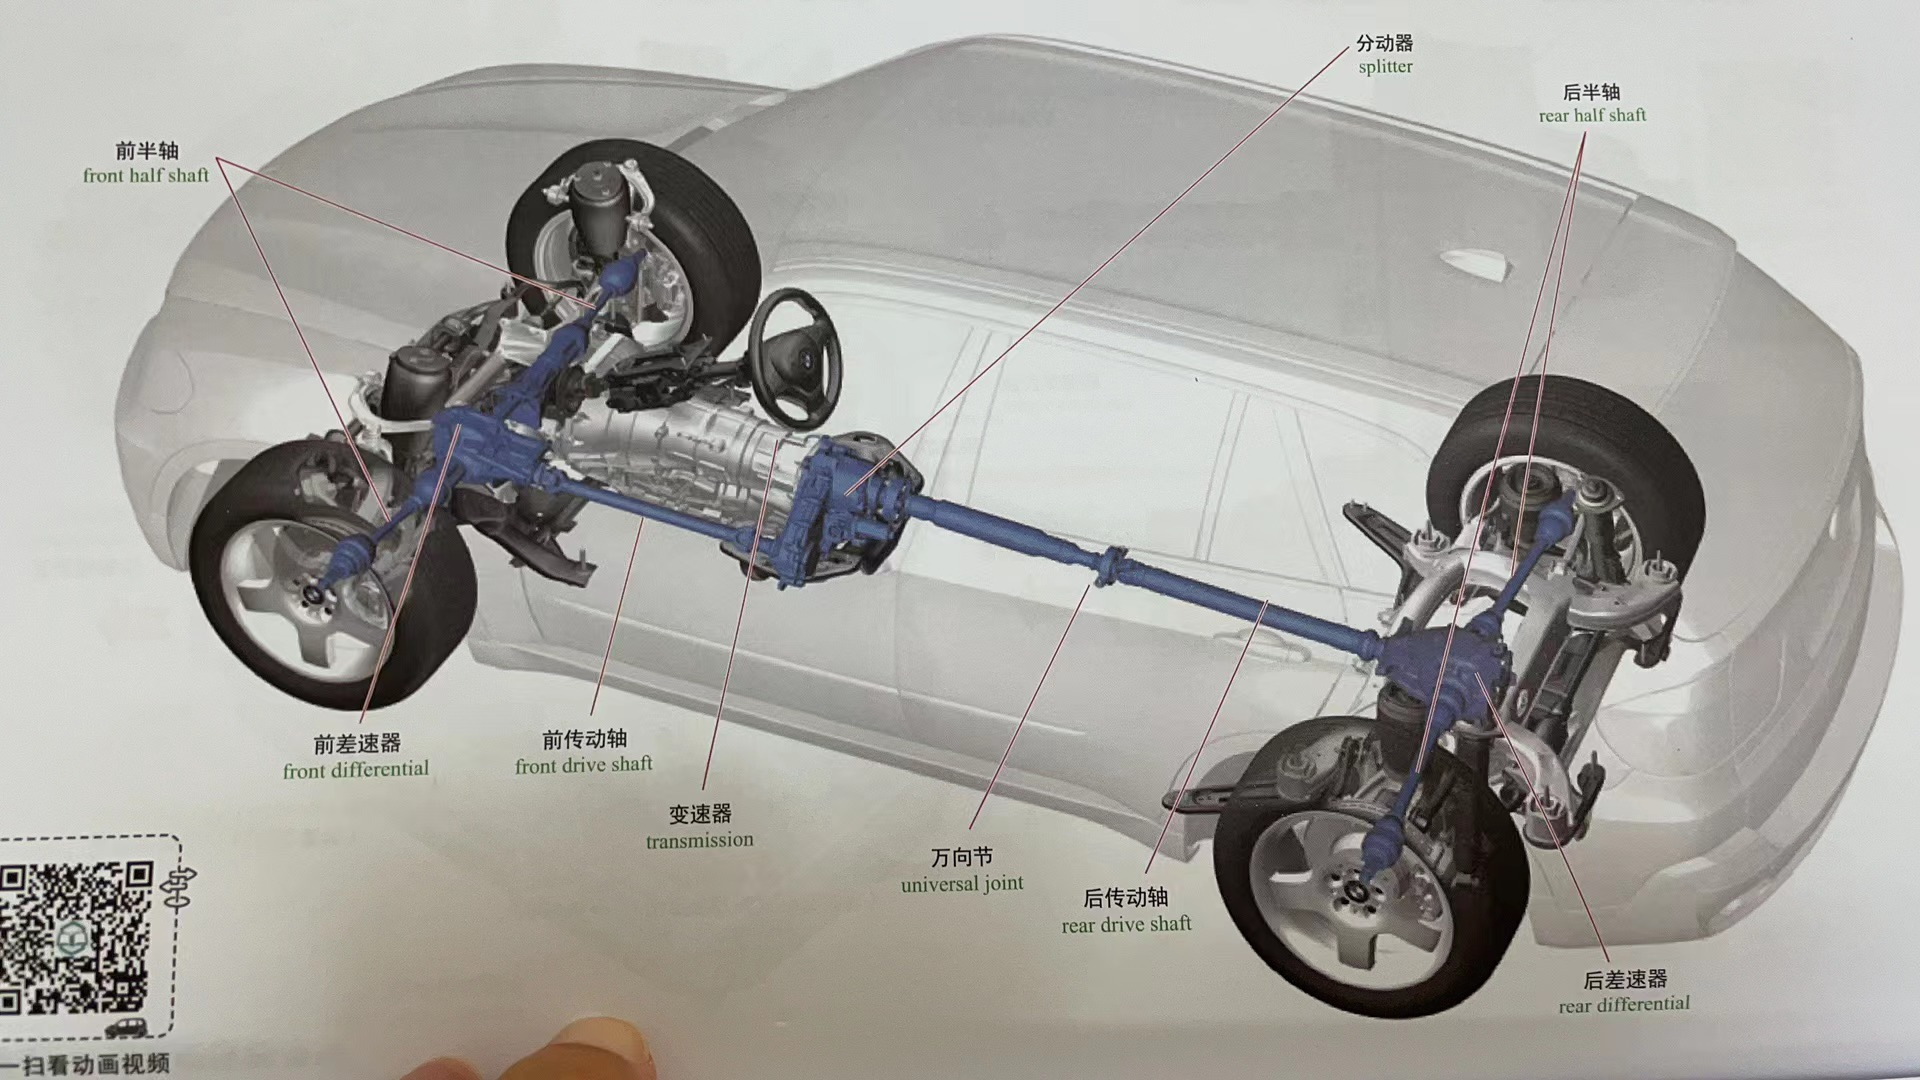
\includegraphics[width=0.5\textwidth]{3-9}
		\begin{enumerate}[label*=\arabic*)]
			\item 种类
				\begin{equation*}
					\begin{cases}
						\text{适时四驱,可以根据实际情况切换为}\begin{cases}
							\text{前二轮驱动} \\
							\text{4轮驱动}
						\end{cases} \\
						\text{全时四驱} \\
						\text{分时四驱(part-time 4WD),由驾驶者手动接通/断开分动器来变换为}\begin{cases}
							\text{前2轮驱动} \\
							\text{后2轮驱动} \\
							\text{4轮驱动}
						\end{cases}
					\end{cases}
				\end{equation*}
			\item 分动器
			
				一般用于四驱(适时四驱一般没有,用来将变速器的动力合理分配给前后传动轴)
			\item 耦合器
			
				一般用于适时四驱。集成在后驱动桥中充当驱动桥的作用。其可以将后轮的状态传递给DIM(dirver information unit),CEM(central electronic module),BCM(brake control module),ECU(电机控制单元)
				\begin{center}
					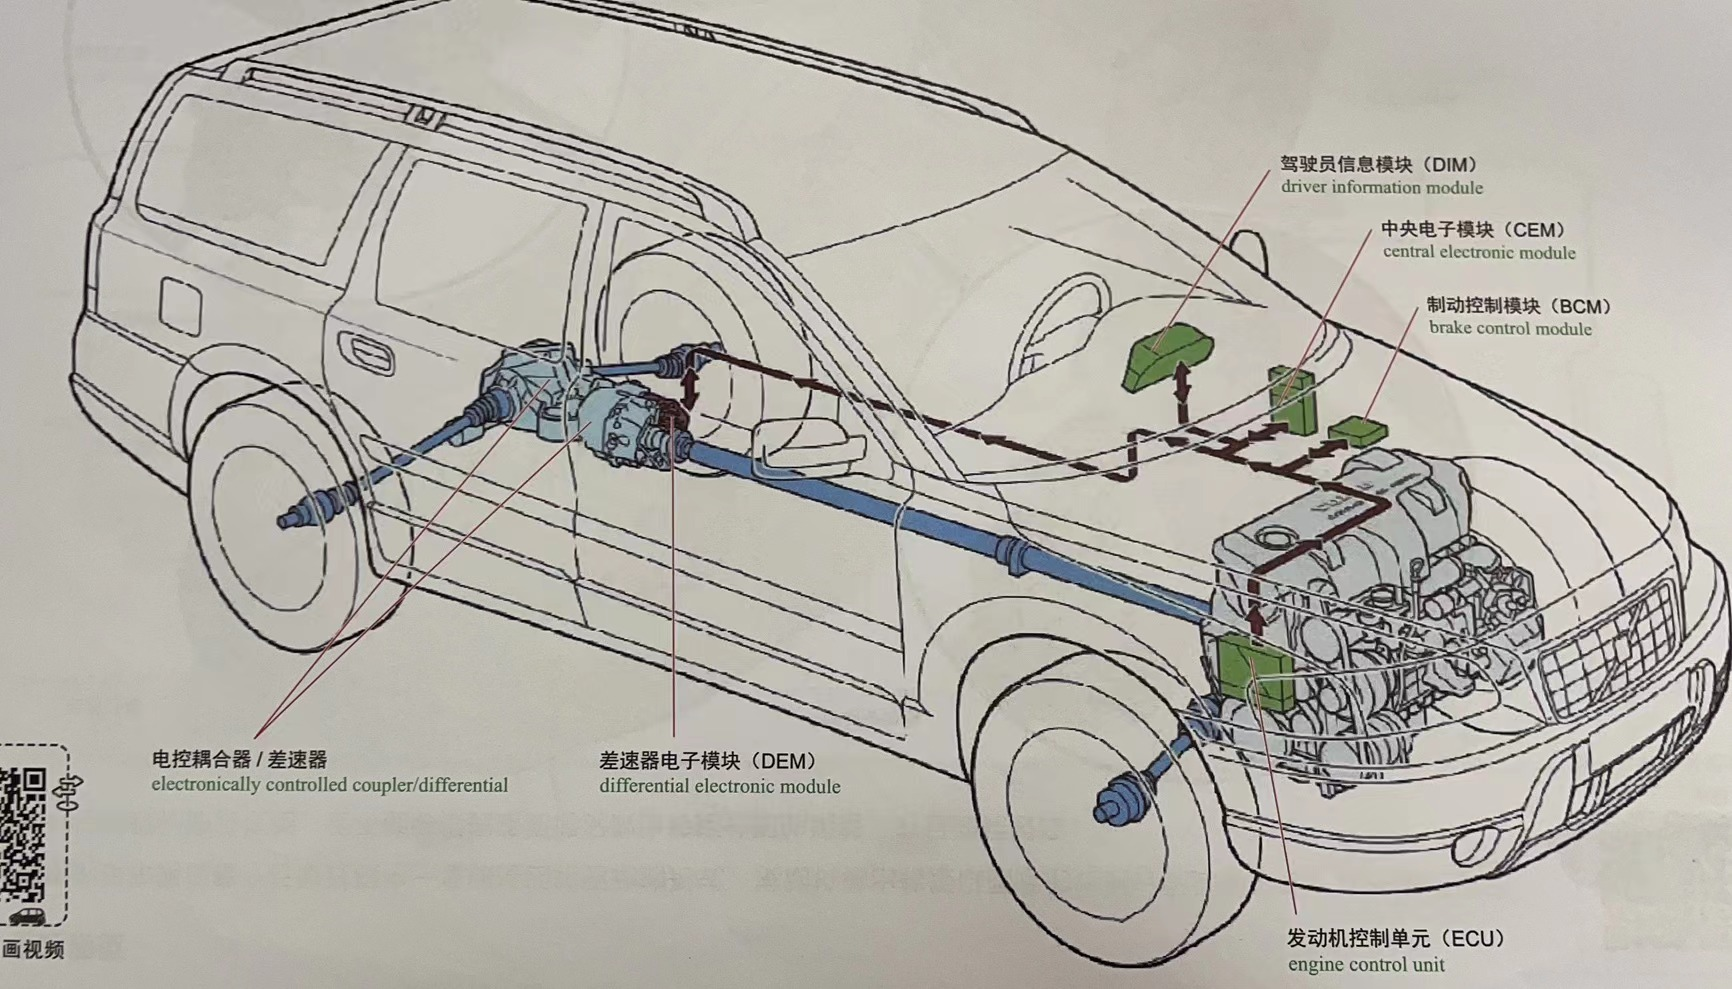
\includegraphics[width=0.5\textwidth]{3-10}
				\end{center}
			\item 传动轴与驱动轴
			
				传动轴组成:轴管、伸缩套、万向节
				
				伸缩套用于调节 the distance between 变速器和驱动桥
				
				万向节用于调节其前后轴的夹角,实现二轴等角速度转动
				
				驱动轴(驱动轮对应的半轴)一般位于差速器和驱动轮之间
				\begin{center}
					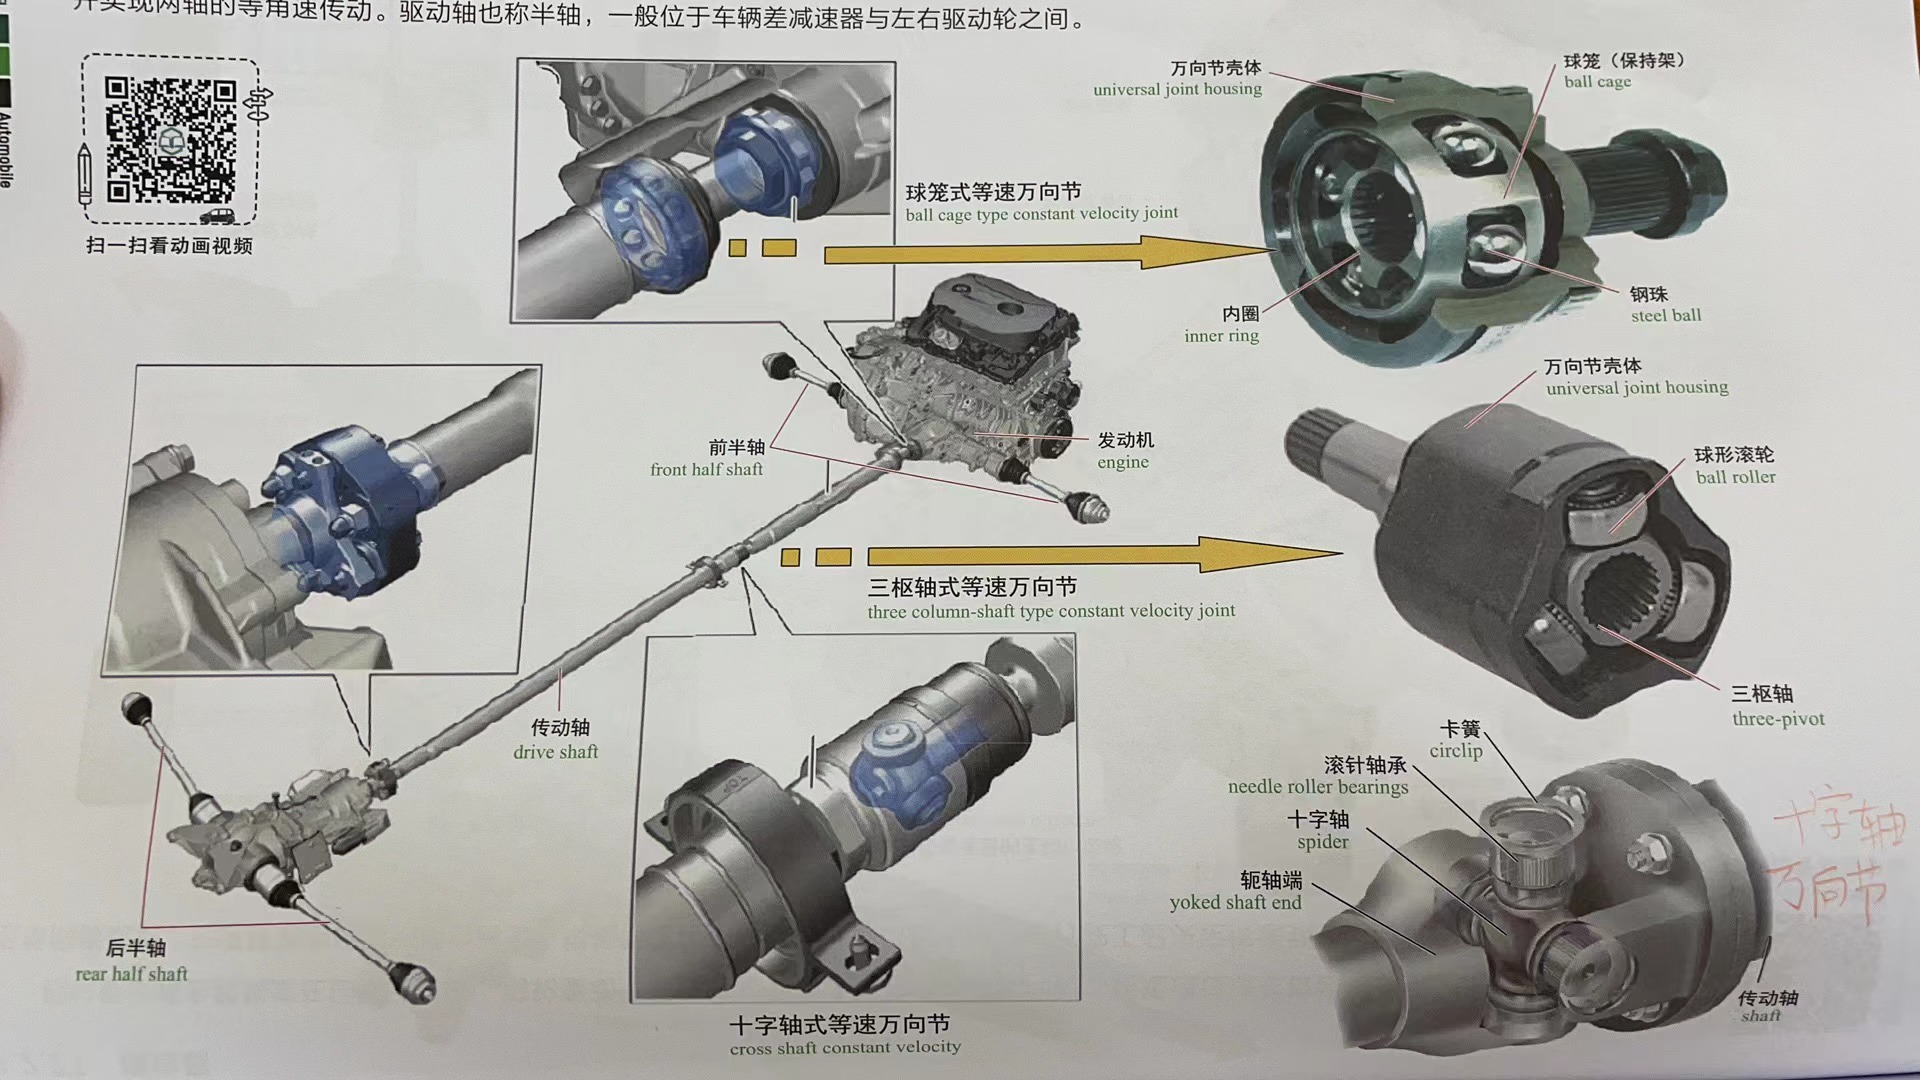
\includegraphics[width=0.5\textwidth]{3-11}
				\end{center}
			\item 差速器与减速器
				差速器:将动力合理分配给左右两车轮
				
				减速器:位于变速器的变速箱中
		\end{enumerate}
\section{行驶系统}
	\subsection{车架}
		车架用于安装车身和底盘的部件
	\subsection{悬架}
		\subsubsection{概述}
			作用:缓冲路面给车架和车身的冲击力;传递车轮和车架之间的力
			
			典型悬架包括弹性元件、导向机构、减震器等
			
			弹性元件又有钢板弹簧、空气弹簧(高级轿车)、螺旋弹簧以及扭杆弹簧(一般轿车常用)
		\subsubsection{类型}
			\begin{equation*}
				\begin{cases}
					\text{独立:一边车轮跳动,另一边车轮不受其影响。包括}\begin{cases}
						\text{双叉臂式} \\
						\text{横臂式} \\
						\text{纵臂式} \\
						\text{多连杆式} \\
						\text{烛式} \\
						\text{麦弗逊式}
					\end{cases} \\
					\text{半独立悬架:如扭杆梁} \\
					\text{非独立:一边车轮跳动,另一边车轮受其影响。轿车不常用,多用于货车、客车。如钢板弹簧悬架}
				\end{cases}
			\end{equation*}
			\begin{center}
				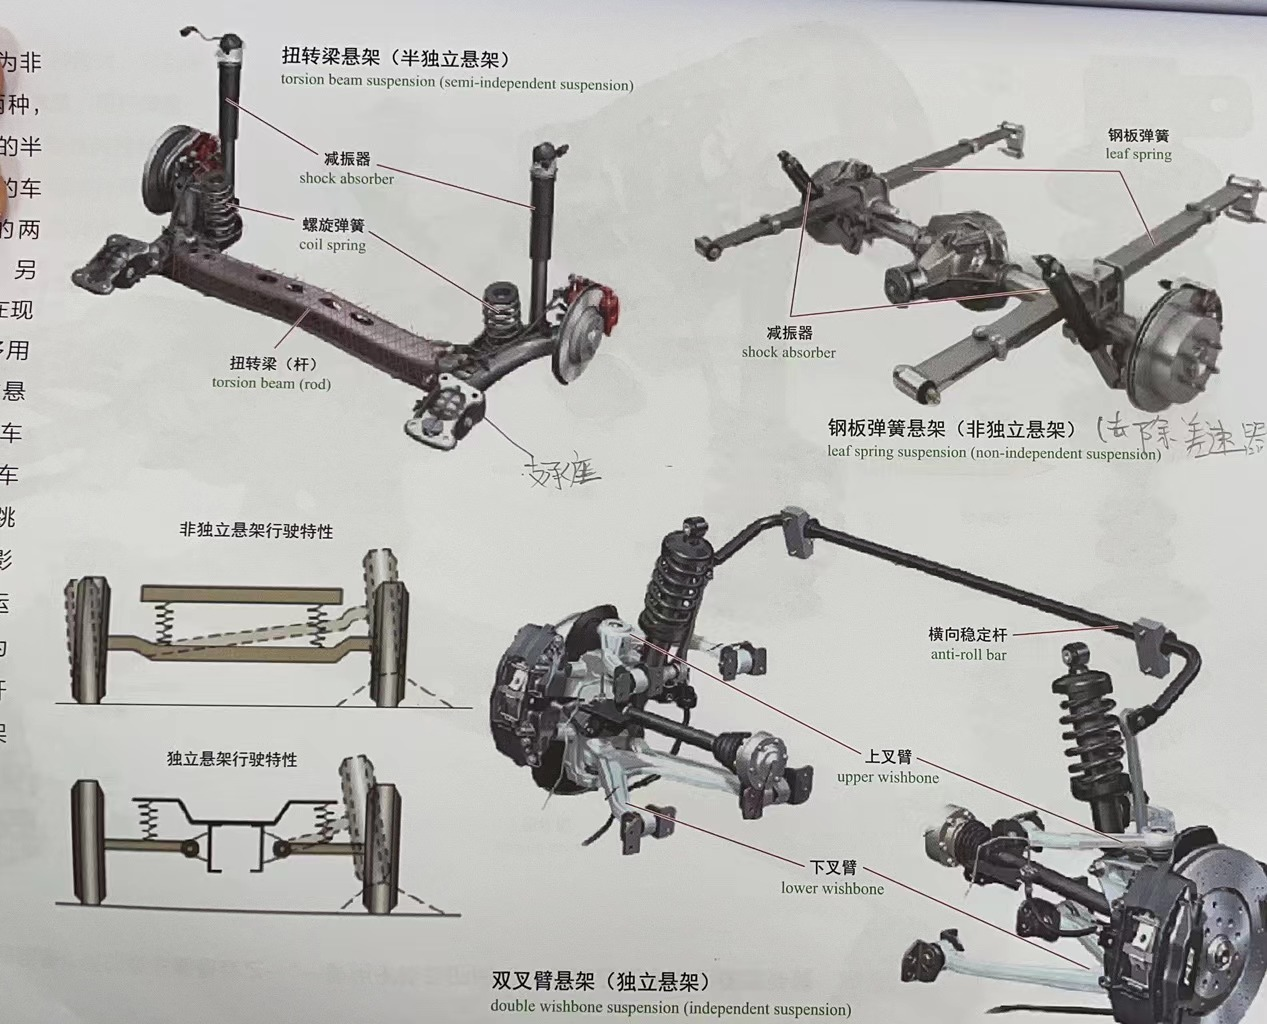
\includegraphics[width=0.5\textwidth]{3-23}
			\end{center}
		\subsection{麦弗逊式悬架}
			\begin{center}
				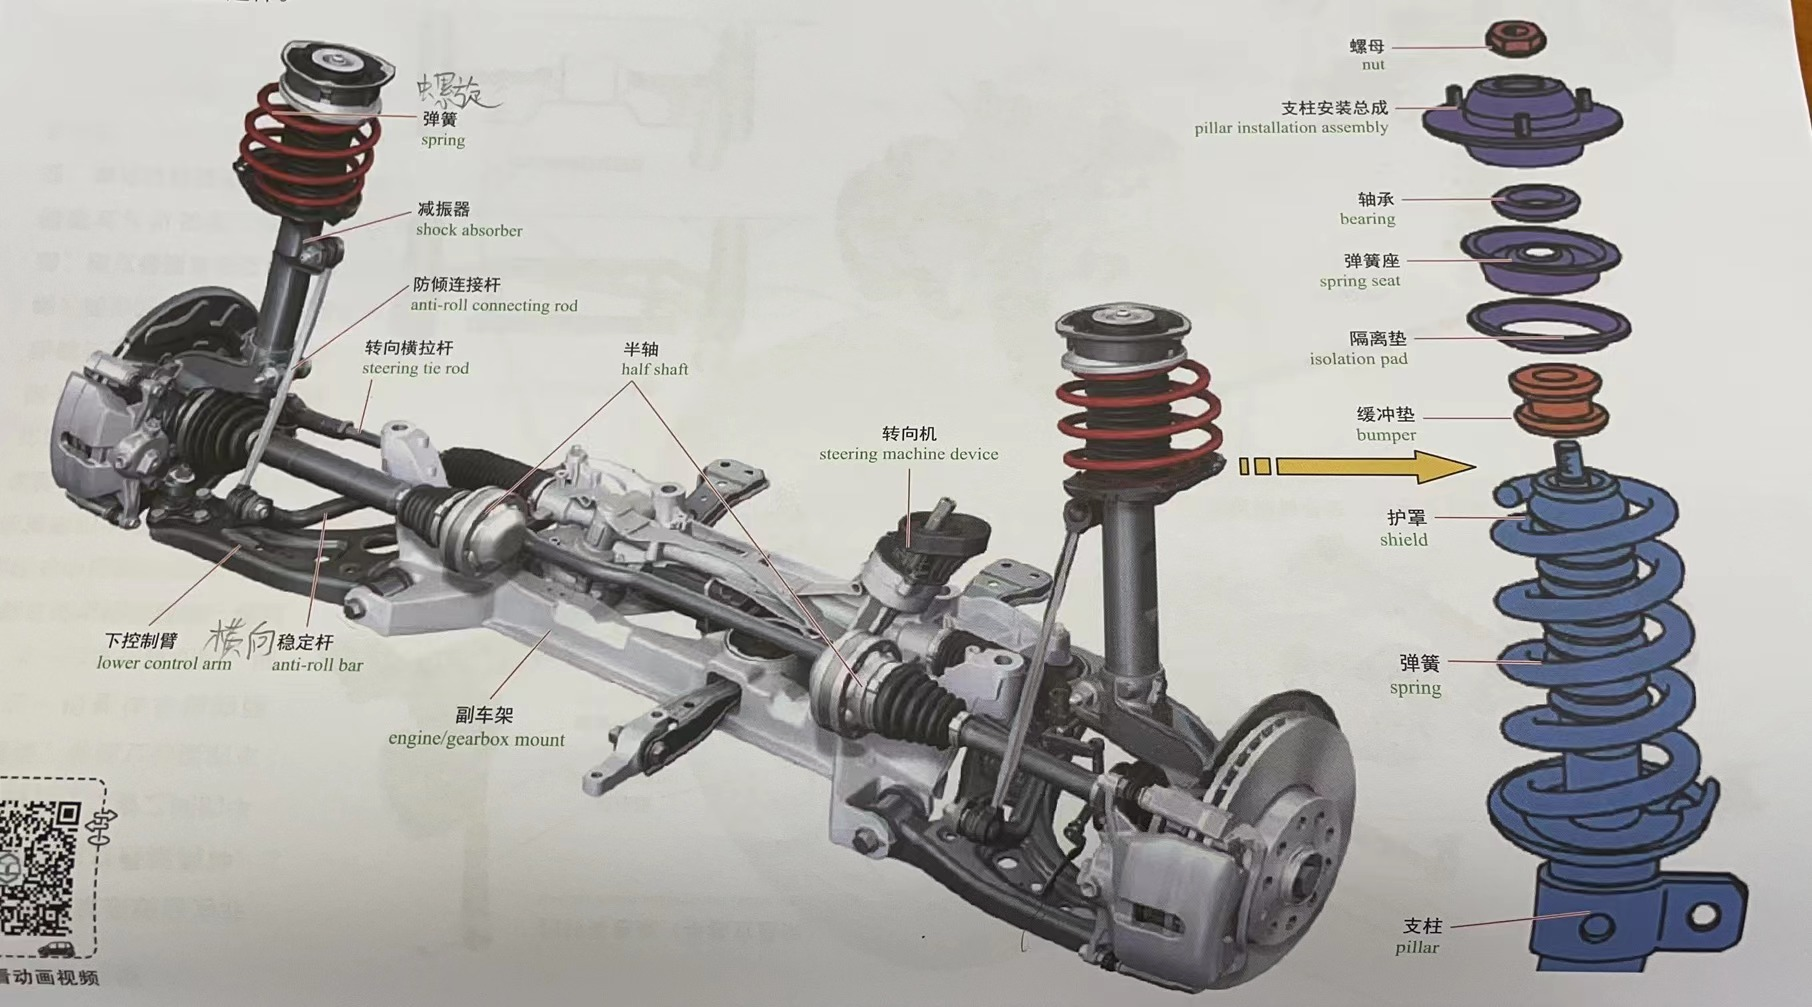
\includegraphics[width=0.5\textwidth]{3-24}
			\end{center}
		\subsection{汽车悬架的弹簧}
			分为螺旋弹簧、钢板弹簧和\underline{扭杆弹簧}$ \begin{cases}
				\text{一端接车架,一端接悬架控制臂} \\
				\text{作用与螺旋弹簧相同}
			\end{cases} $
		\subsection{多连杆悬架(独立悬架)}
			一般连杆(包括控制臂、定位臂在内的杆件)$ \ge $3的悬架
			
			多连杆悬架组成部分$ \begin{cases}
				\text{多连杆前悬架(3/4杆)} \\
				\text{多连杆后悬架(4/5杆)}
			\end{cases} $
			\begin{center}
				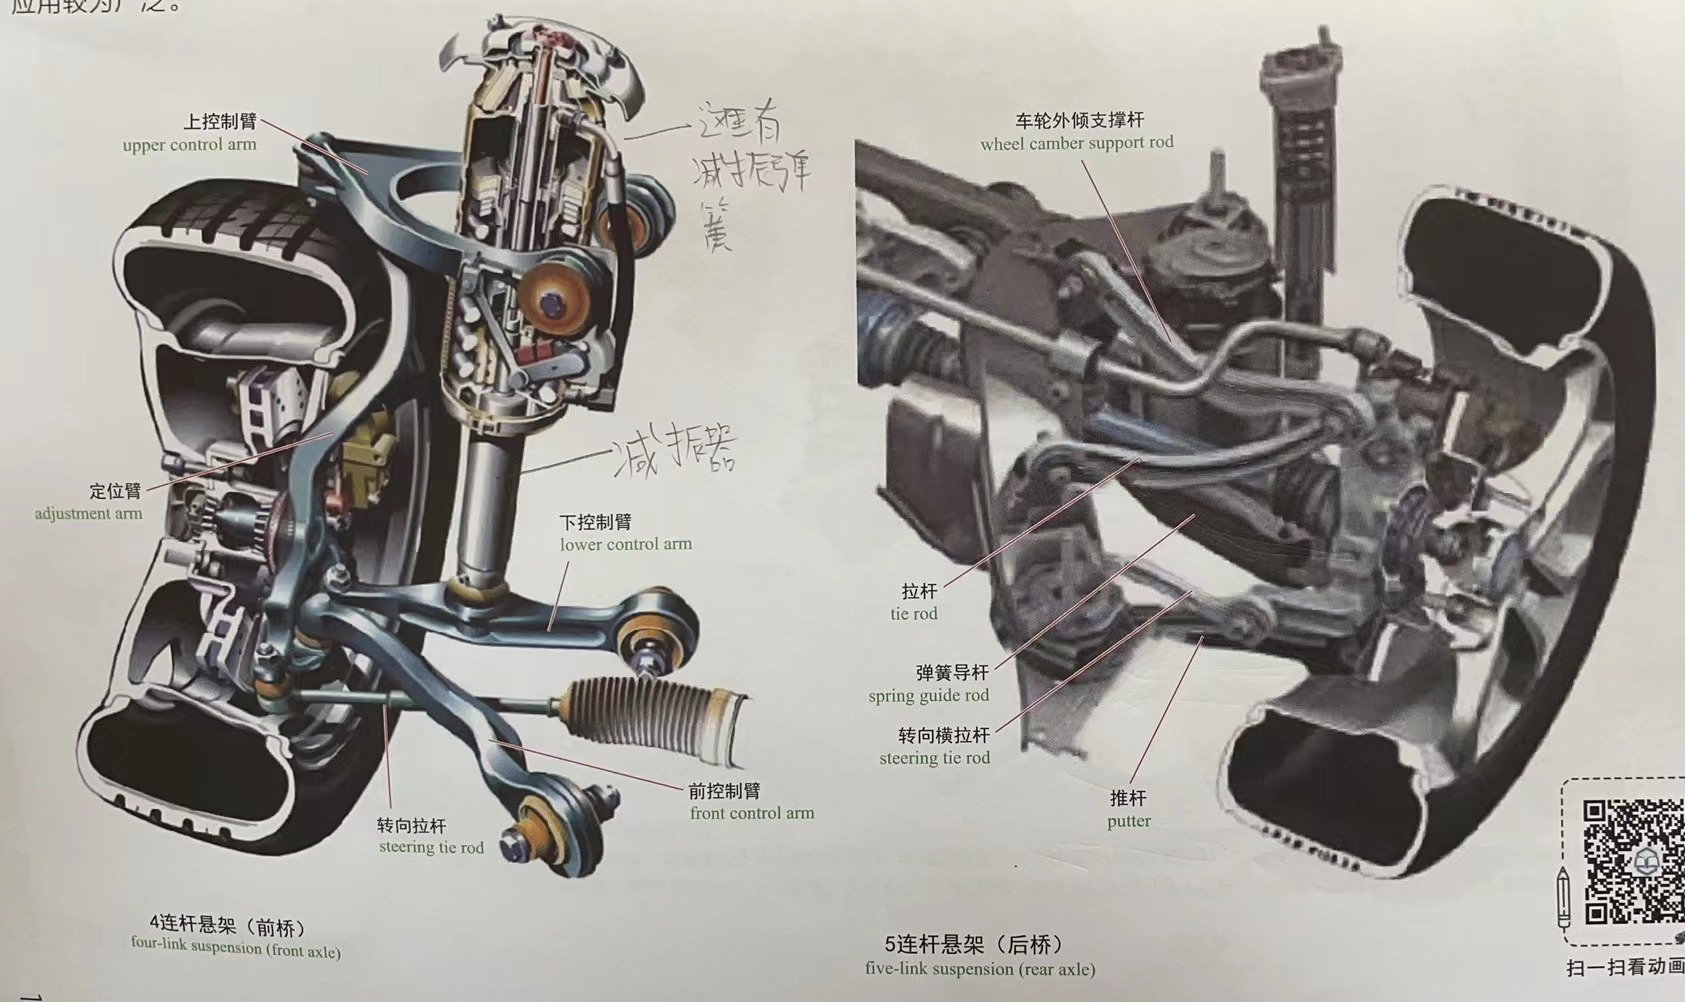
\includegraphics[width=0.5\textwidth]{3-25}
			\end{center}
		\subsection{稳定杆和减振器}
			\begin{enumerate}[label*=\arabic*)]
				\item 减振器不包括螺旋弹簧,但螺旋弹簧可以固定在减震器上。螺旋弹簧用于吸收地面的冲击。减震器用于加速车架车身振动衰减以改善汽车行驶的平顺性。
				\item 减震器种类:
					
					筒式减振器(可以指螺旋弹簧振荡)、充气式减振器、阻尼可调式减振器
				\item 横向稳定杆(防倾杆、平衡杆)用于防止车身在转弯时发生过大的横向侧倾(车身侧倾时悬架左右两侧跳动不一致,外侧悬架会压向稳定杆,内侧悬架从而被悬架压住)
				\begin{center}
					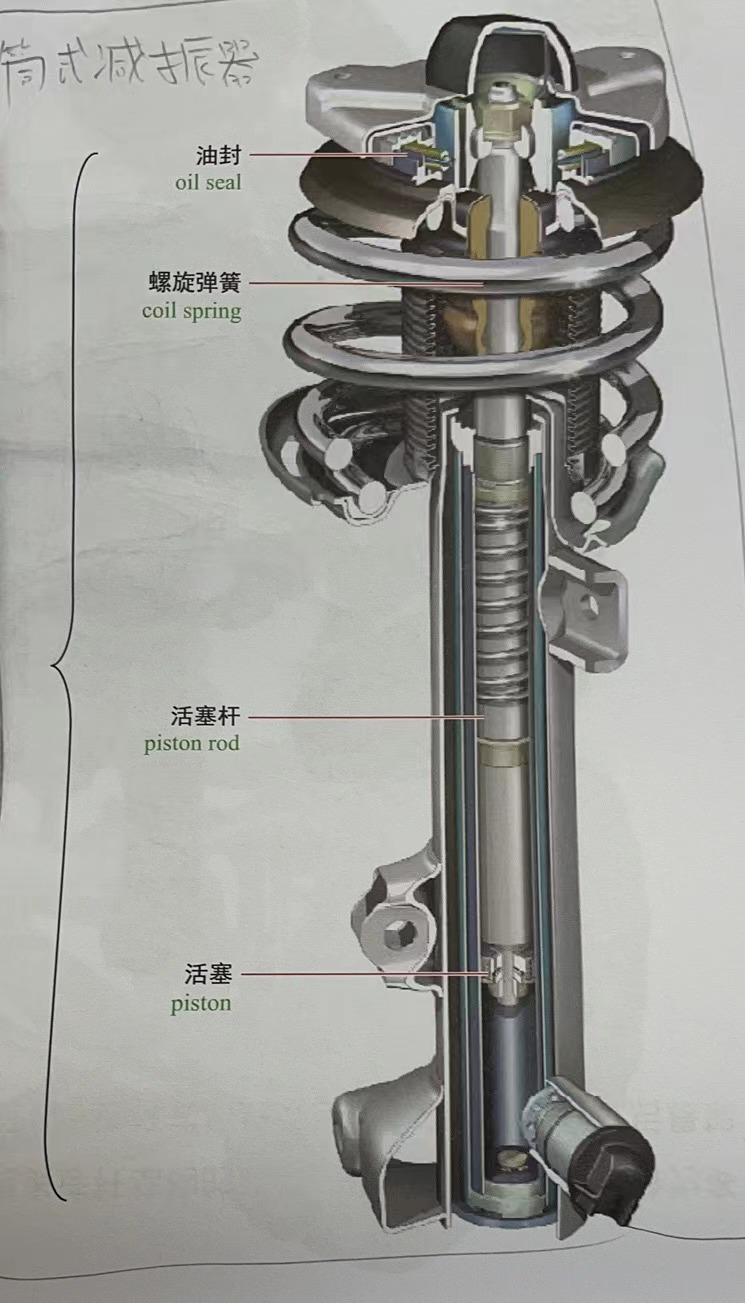
\includegraphics[width=0.5\textwidth]{3-26}
				\end{center}
			\end{enumerate}
		\subsection{空气悬架}
			使用空气减震器的悬架
			
			空气悬架通过充放气实现车身的抬高和降低。行驶时抬高车身能提高通过性;降低时重心降低,提高稳定性。停车时降低有利于上下车。
			
			\begin{center}
				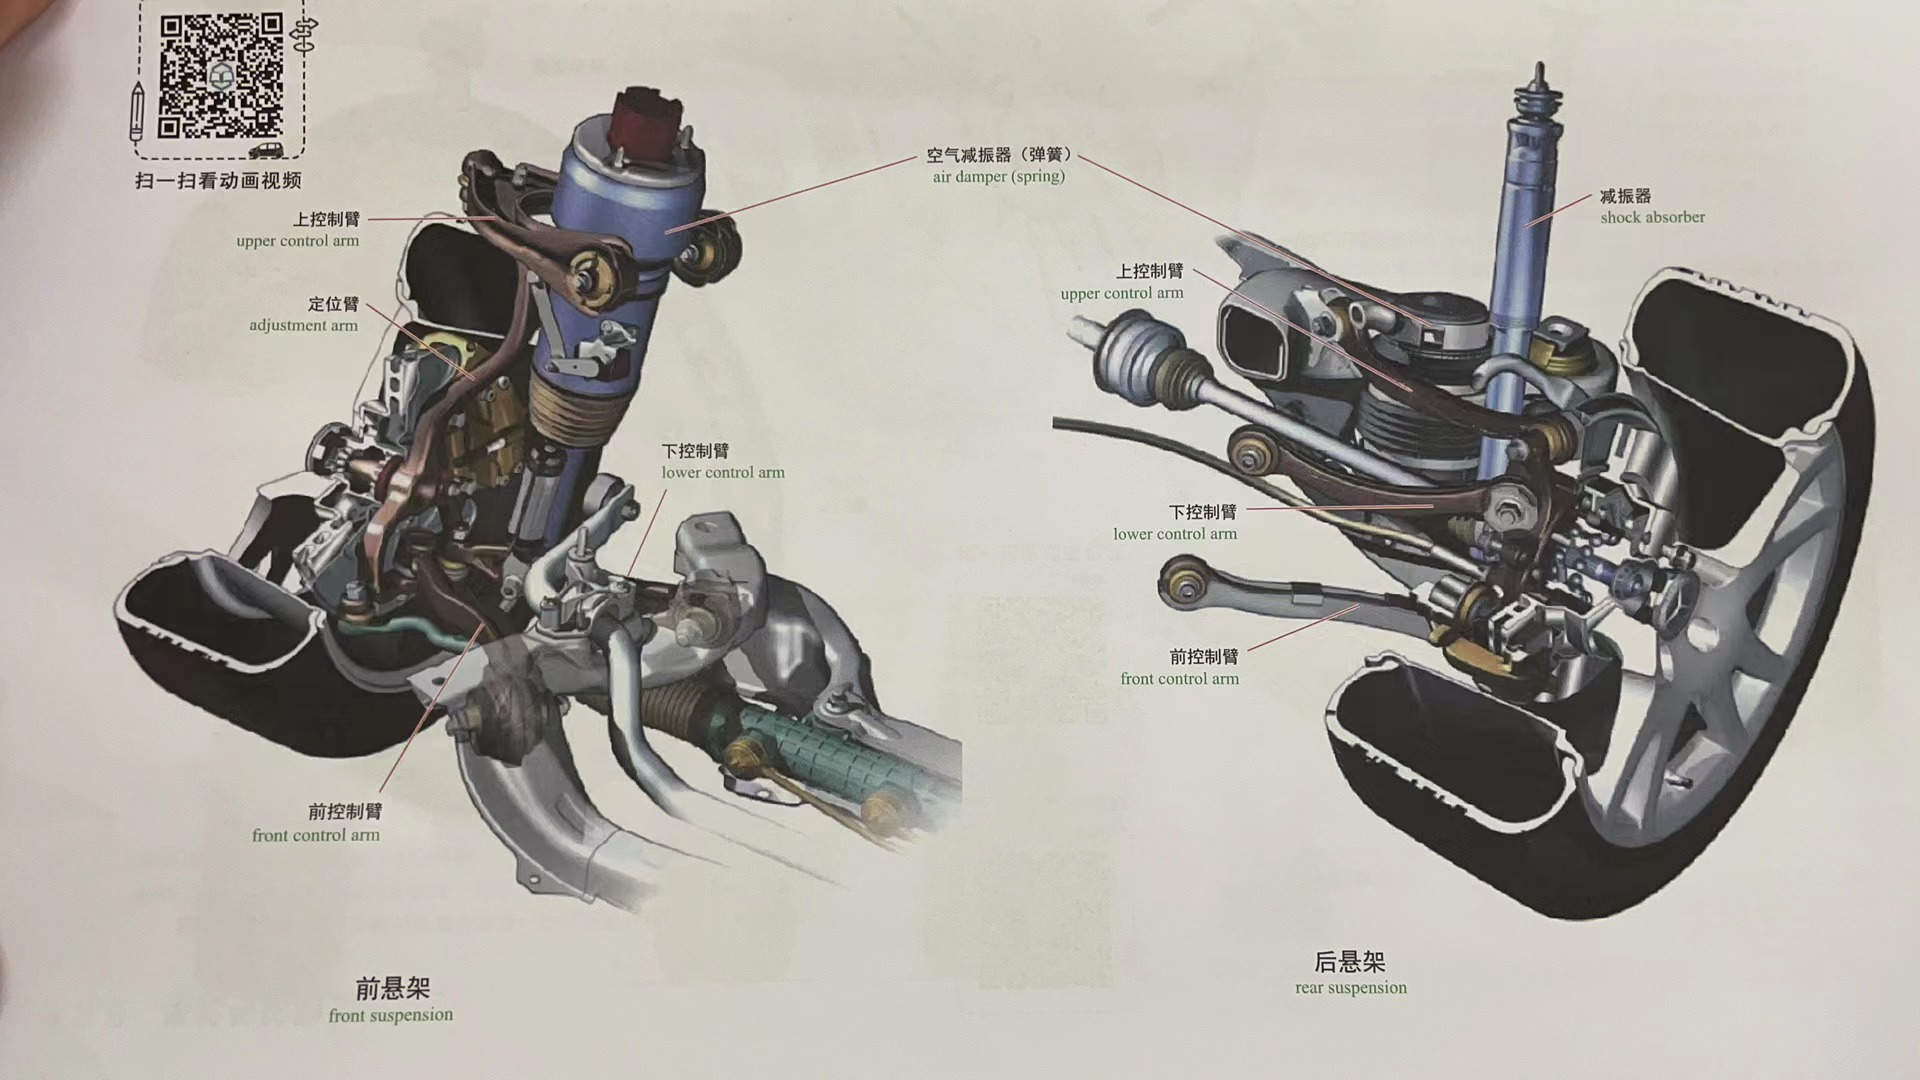
\includegraphics[width=0.5\textwidth]{3-27}
			\end{center}
		
		\subsection{车轮}
			由轮辋和轮辐组成,不包括轮毂(连接车轮和半轴)
				\[ 195(\text{断面宽度W})/60(\text{扁平比AR})\quad R14(\text{轮辋直径})\quad 85(载重指数)\quad H(\text{}速度级别) \]
				\[  \text{扁平比} = \dfrac{\text{断面高度H}}{\text{断面宽度W}}\%\]
					
			车轮定位:使车轮、转向机构、前后轴的安装应保持一定相对位置的安装
			\subsubsection{前轮定位}
				参数包括:主销后倾角、主销内倾角、前轮外倾角和前轮前束
				\begin{itemize}
					\item 主销后倾角
						\begin{description}
							\item[作用]在车轮受外力向外偏转时施加一个回正力矩,使车轮自动回正
								\begin{center}
									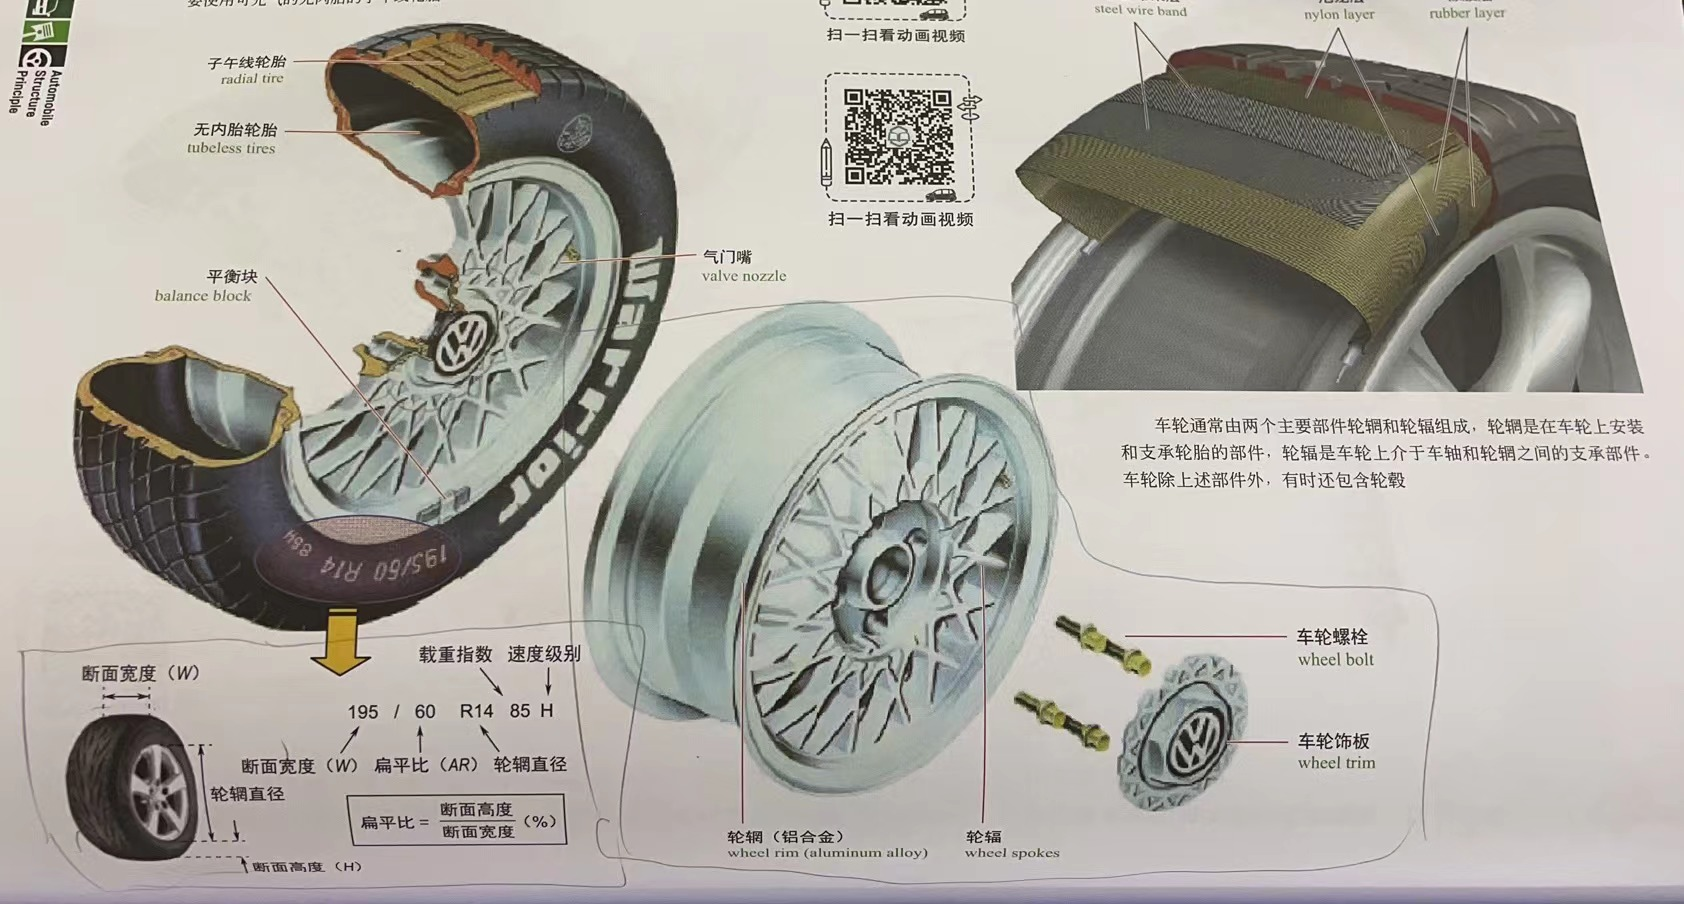
\includegraphics[width=0.3\textwidth]{3-28}
								\end{center}
						\end{description}
					\item 主销内倾角
						\begin{description}
							\item[作用] 转向轻便、减少车轮回跳和跑偏(可以改善汽车直线行驶的稳定性)
							\item[危害] 主销内倾角过大,会加剧轮胎转向时的磨损
								\begin{center}
									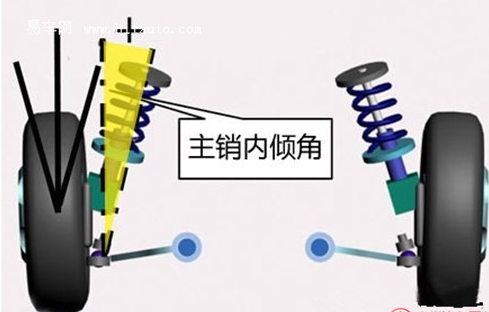
\includegraphics[width=0.3\textwidth]{3-29}
								\end{center}
							\item[偏距]							
								\begin{center}
									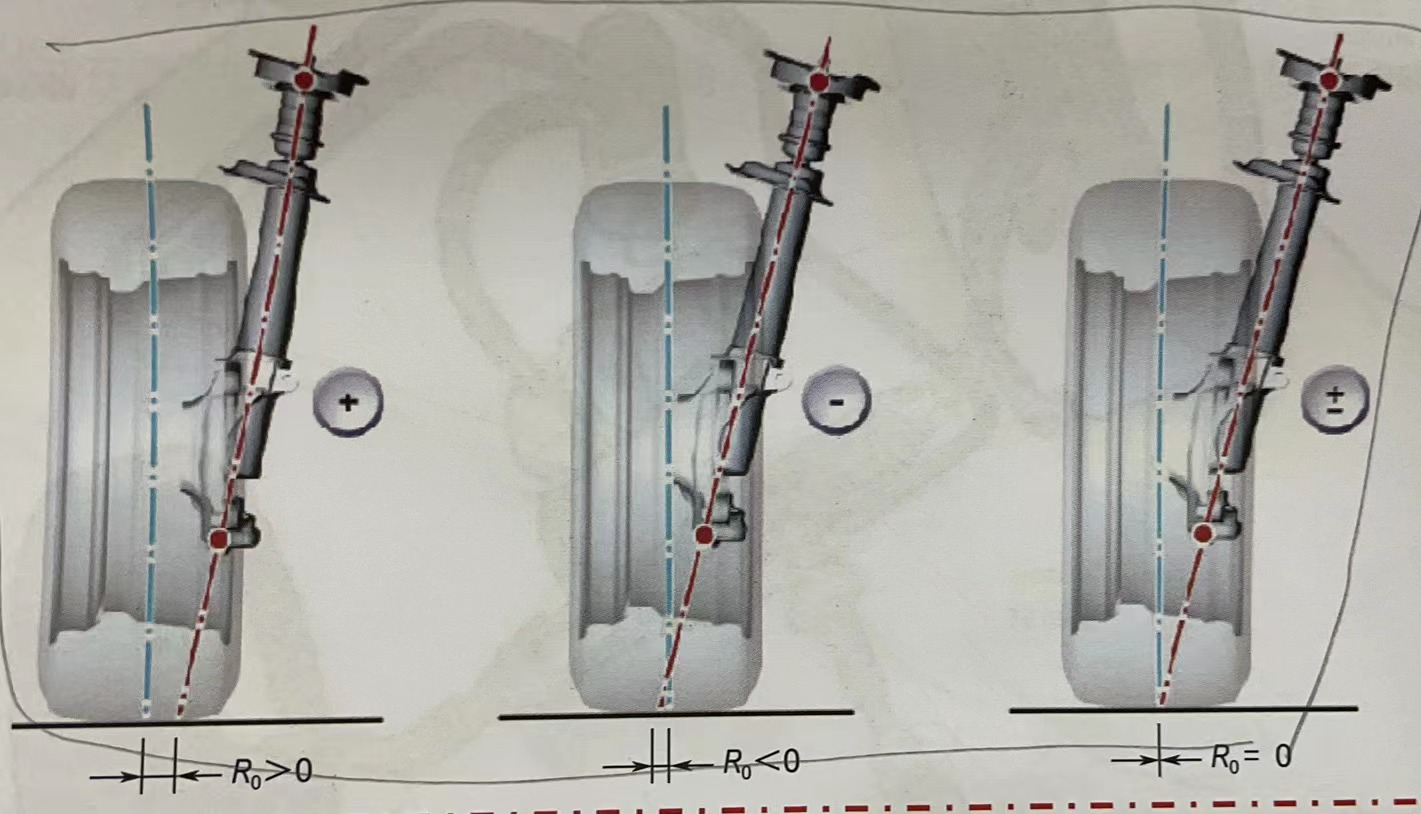
\includegraphics[width=0.5\textwidth]{3-30}
								\end{center}
						\end{description}
					\item 前轮外倾角
								\begin{enumerate}
									\item 在汽车负载时让车轮保持垂直,从而减少轮胎磨损,提高行驶的安全性、稳定性和舒适性
									\item 使车轮更靠近轮毂内侧,减少外轴承和轮毂螺母的负荷(减少外轴承的负荷可以减少转向阻力)
								\end{enumerate}
							\begin{center}
								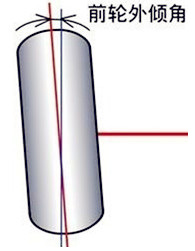
\includegraphics[width=0.15\textwidth]{3-31}
							\end{center}
					\item 前轮前束
						\begin{description}
							\item[内束] 前轮向内收束。作用为给车轮增加一个向内滚动的趋势,抵消车轮外倾给车轮增加的向外滚动的趋势,使车轮向前滚动
							\item[外束] ~
						\end{description}
						\begin{center}
							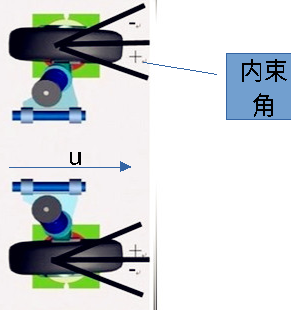
\includegraphics[width=0.3\textwidth]{3-32}
						\end{center}
				\end{itemize}
\section{转向系统}
\subsection{概述}
	一般由转向机、传动机构与操纵(控制)机构组成。
	
	常用的转向机:齿轮齿条式和循环球式
	
	种类:液压助力转向系统,电动助力转向系统
	
		\begin{figure}[htbp]
			\centering
			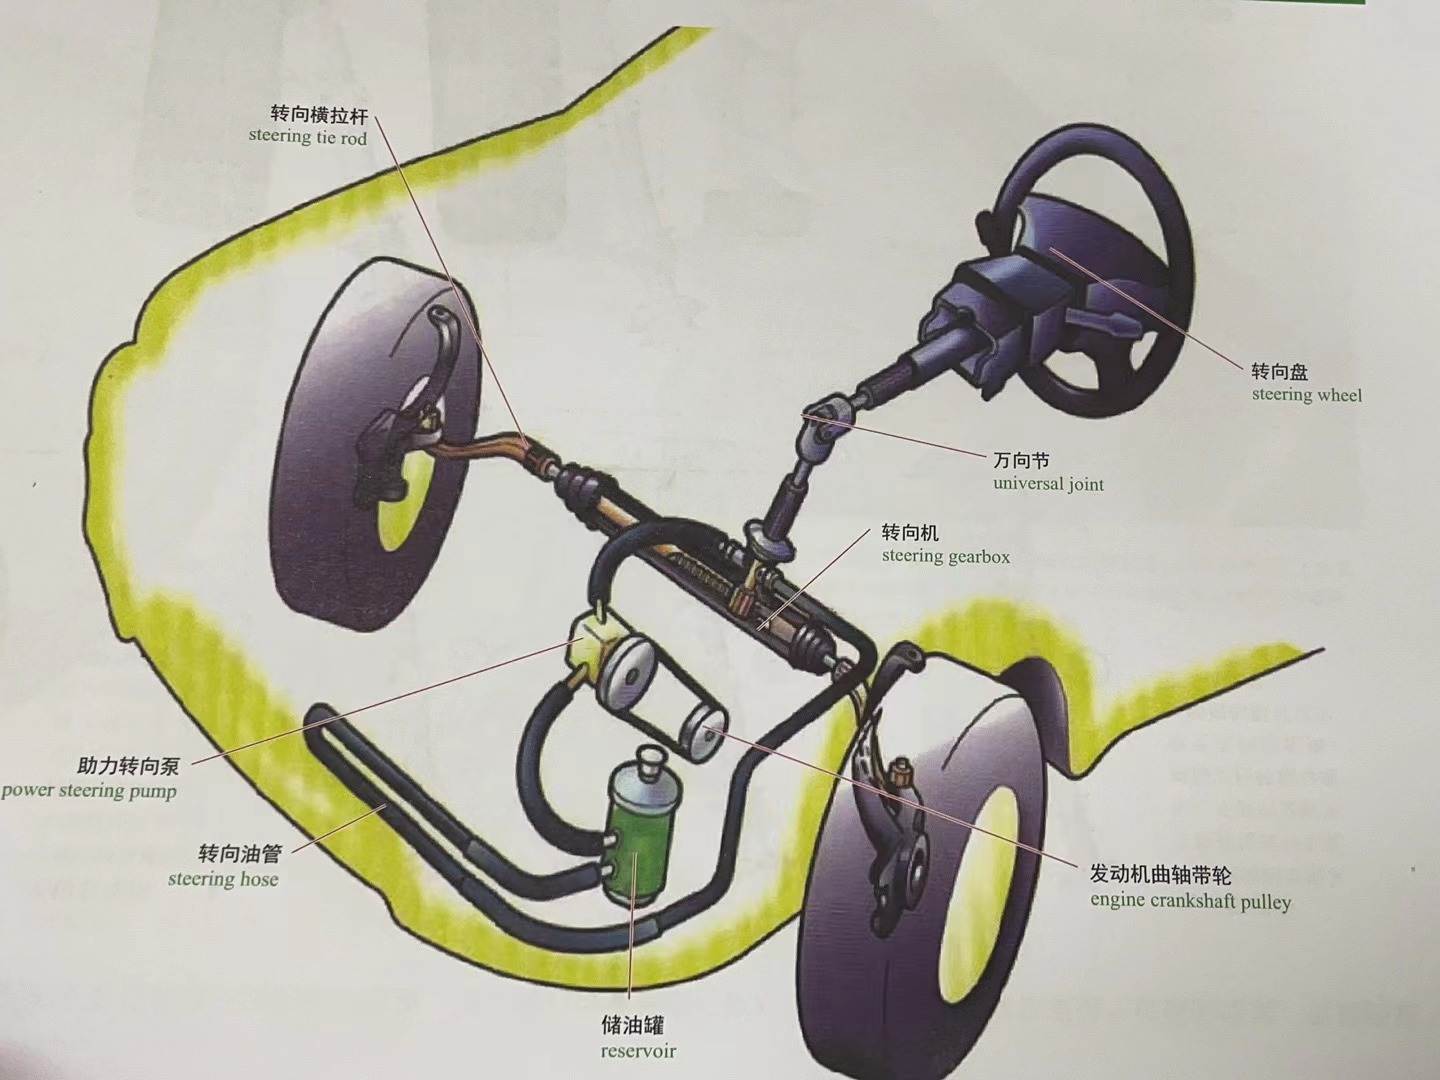
\includegraphics[width=0.5\textwidth]{3-33}
		\end{figure}
\subsection{齿轮齿条式转向机(多用于货车)}
	\begin{figure}[htbp]
		\centering
		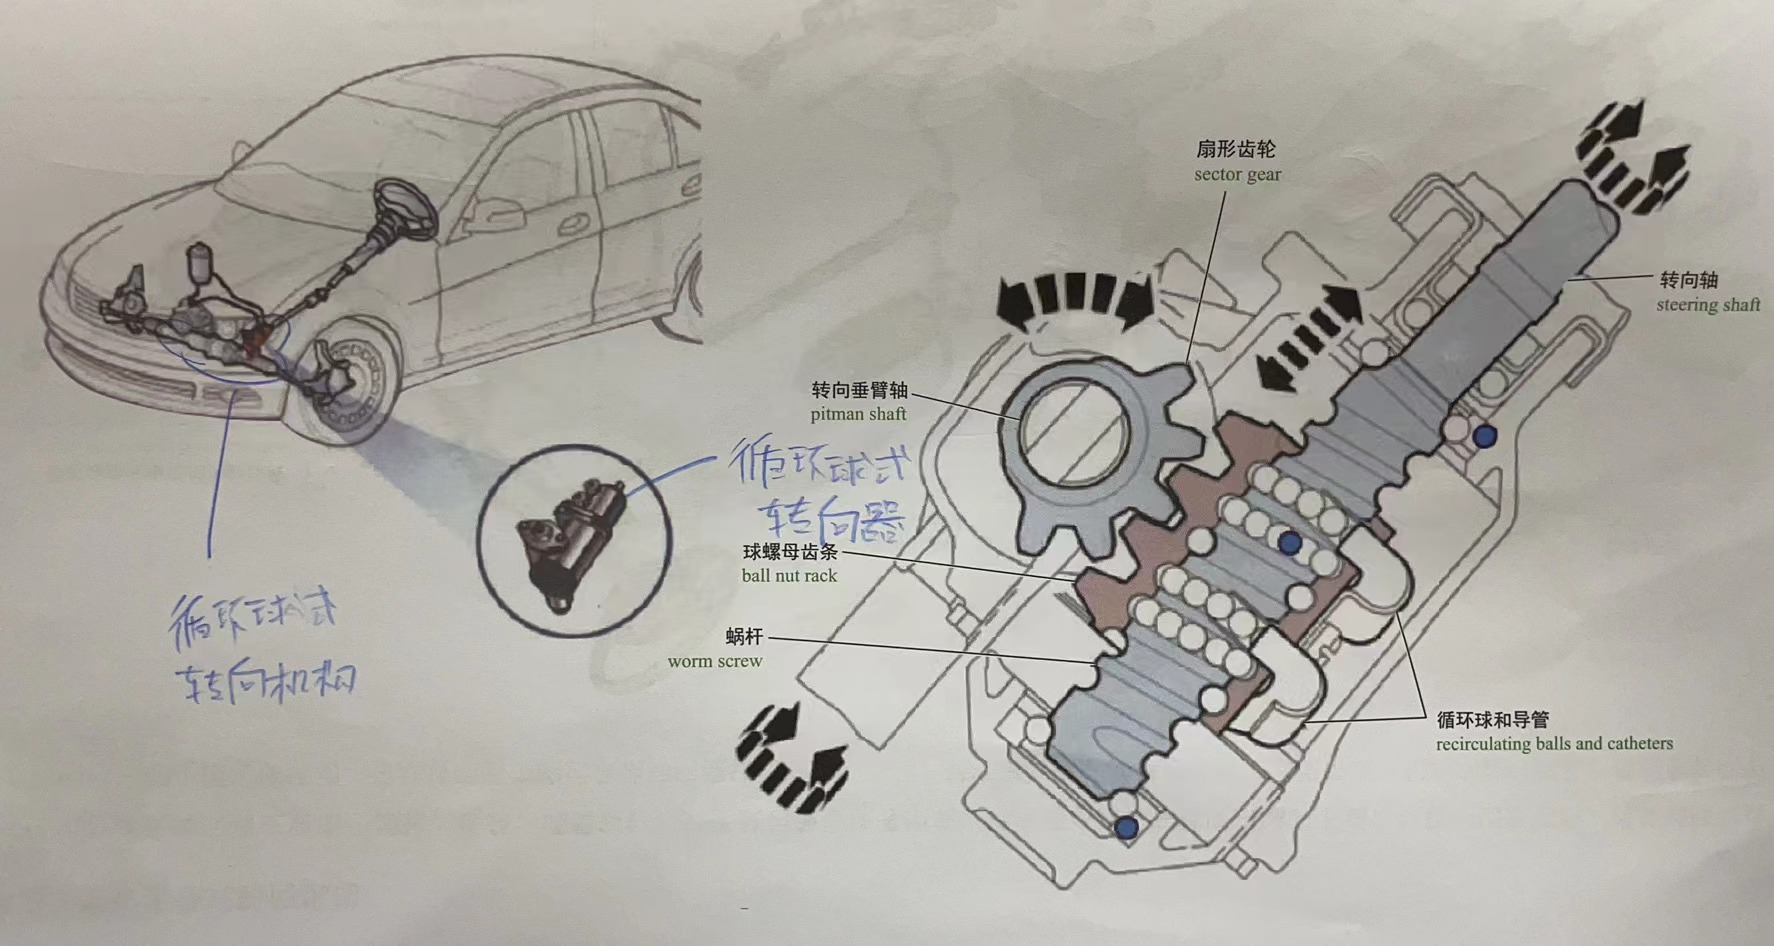
\includegraphics[width=0.5\textwidth]{3-34}
	\end{figure}
\subsection{齿轮齿条式转向机}
	\begin{figure}[htbp]
		\centering
		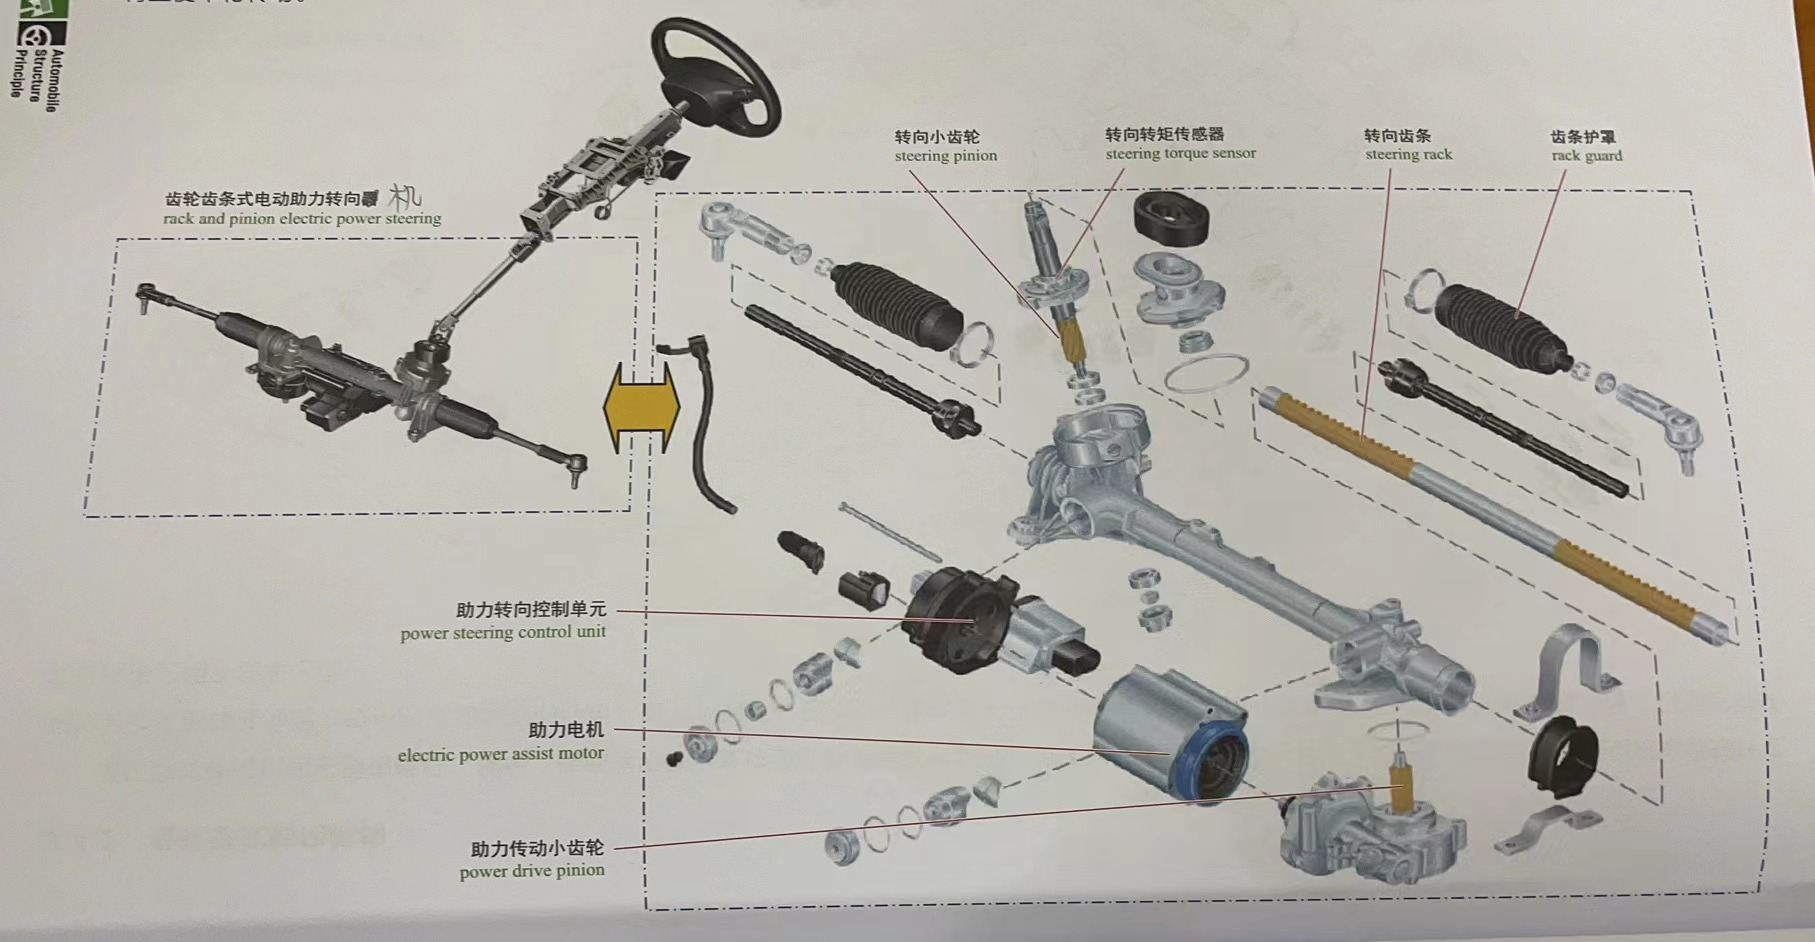
\includegraphics[width=0.5\textwidth]{3-35}
	\end{figure}
\subsection{液压助力转向系统}
	液压泵通过油路传递转向助力
	
	机械式、电动式
	
	
	\begin{figure}[htbp]
		\centering
		\caption*{\normalsize 机械式原理:发动机带动液压泵,液压泵推动活塞,活塞推动转向拉杆}
		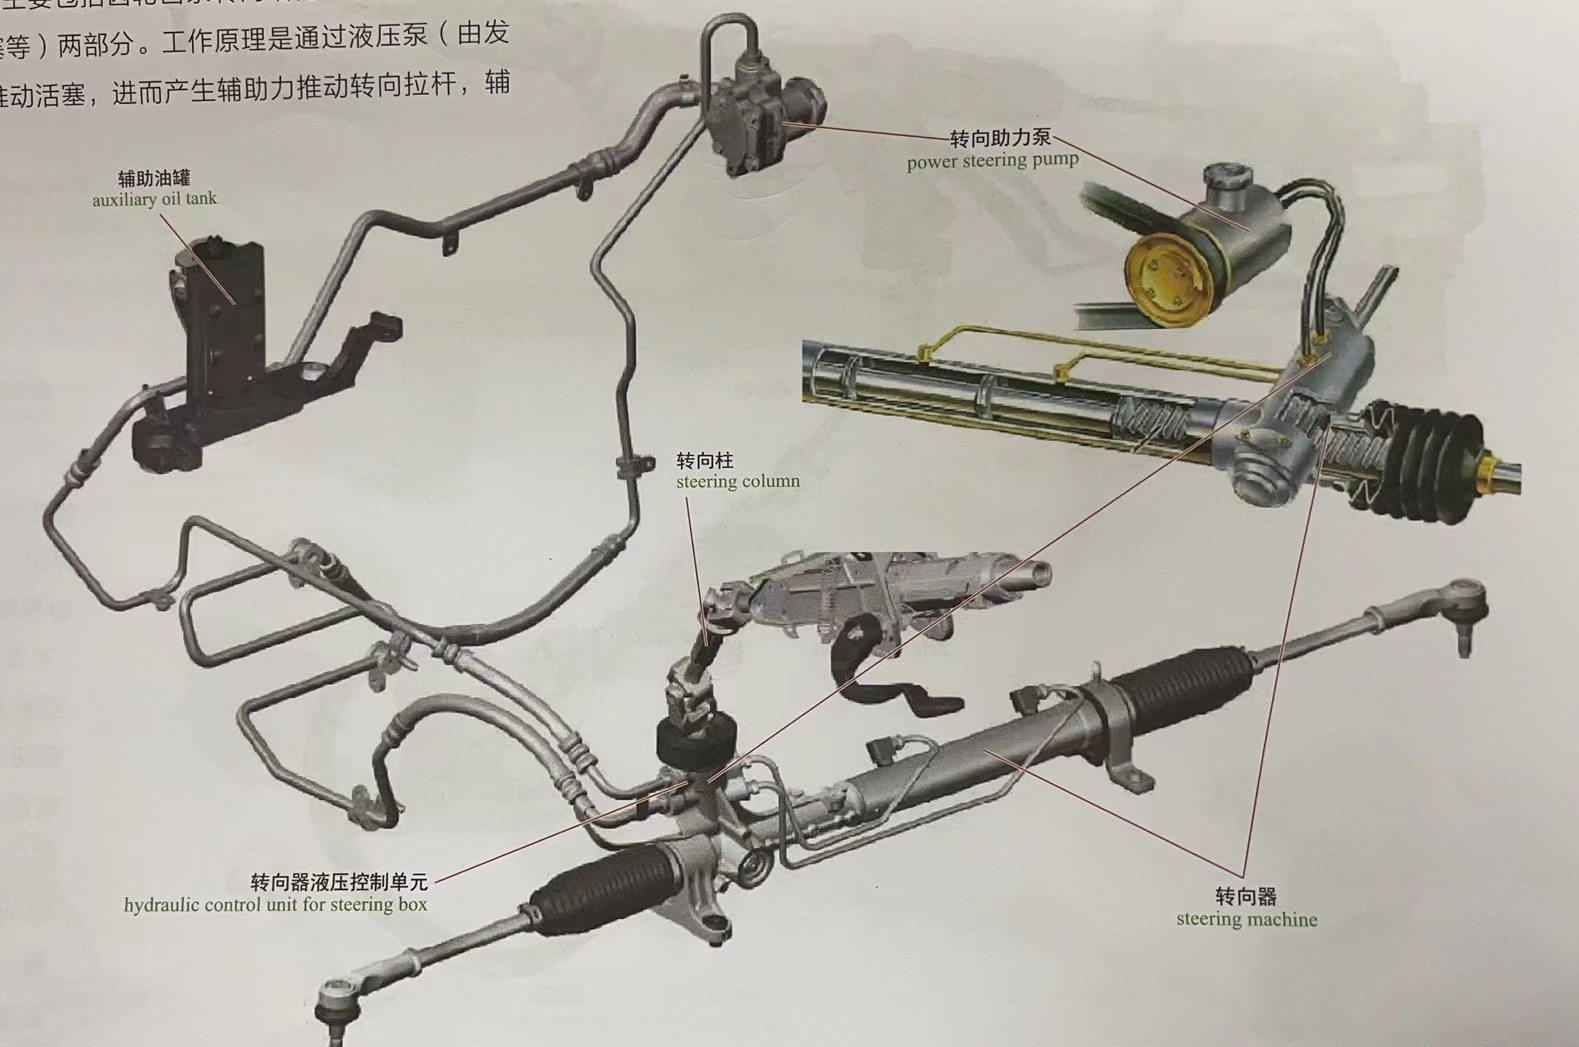
\includegraphics[width=0.5\textwidth]{3-36}
	\end{figure}

	
	\begin{figure}[htbp]
		\centering
		\caption*{\normalsize 电动式原理:电子泵...}
		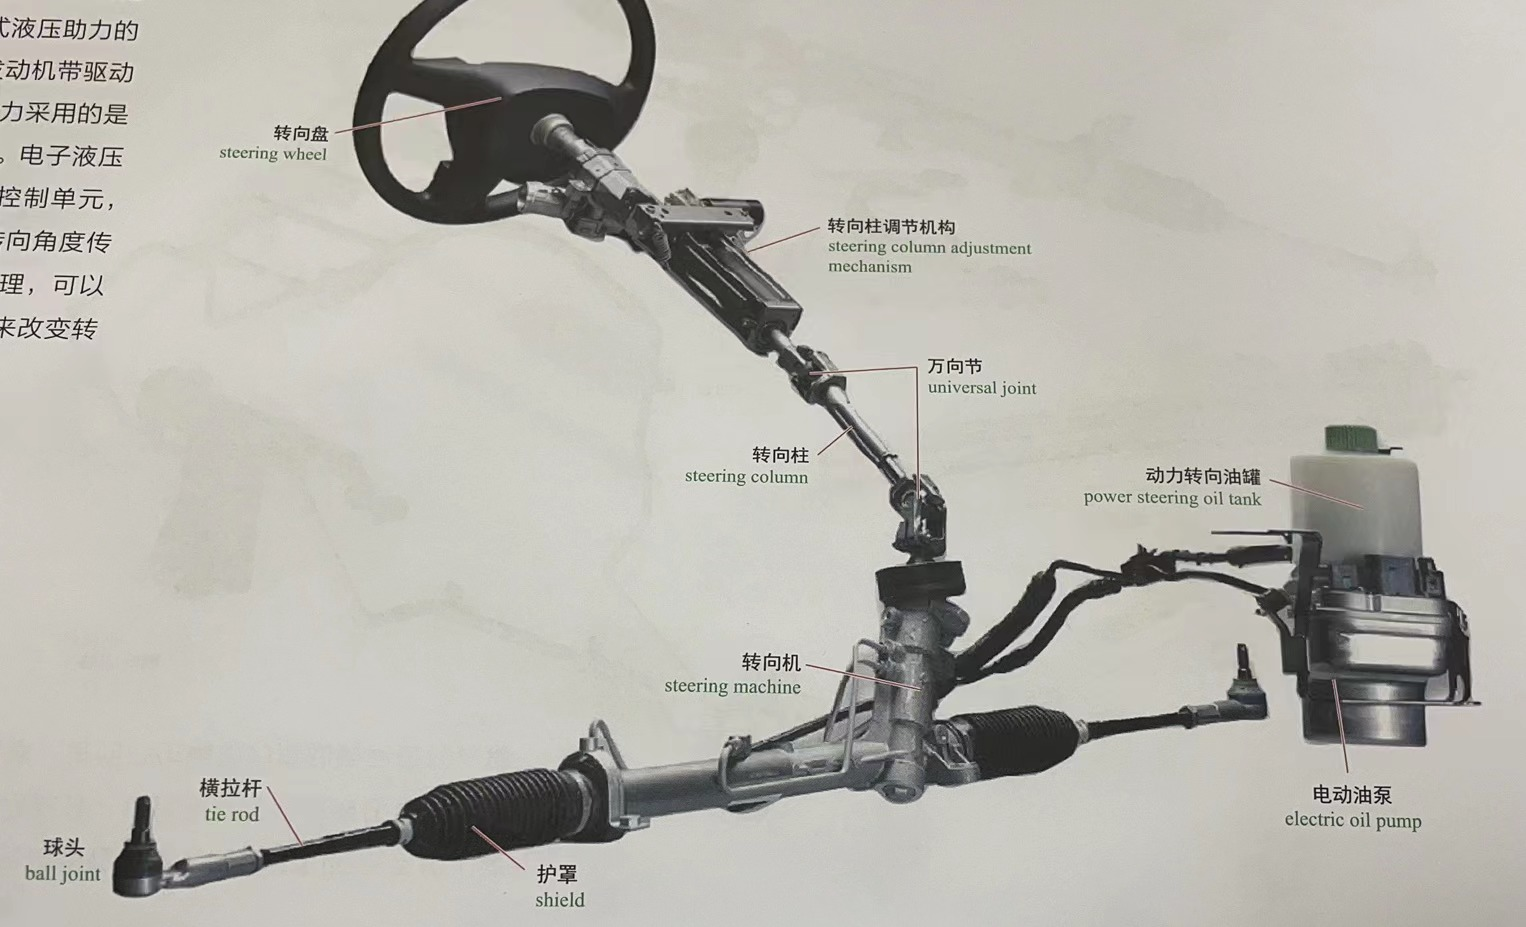
\includegraphics[width=0.5\textwidth]{3-37}
	\end{figure}
	
	电动式的电控单元可以改变电子泵的流量 to 改变转向助力的力度 based on 车速传感器、转向角度传感器提供的数据
	
\subsection{电动助力转向系统(EPS, electric power steering)}
	电机直接提供转向助力,不需要油路
	
	根据电机安装位置不同可分为:C-EPS(转向轴助力式), P-EPS(齿轮助力式),R-EPS(齿条助力式)
	\begin{figure}[htbp]
		\centering
		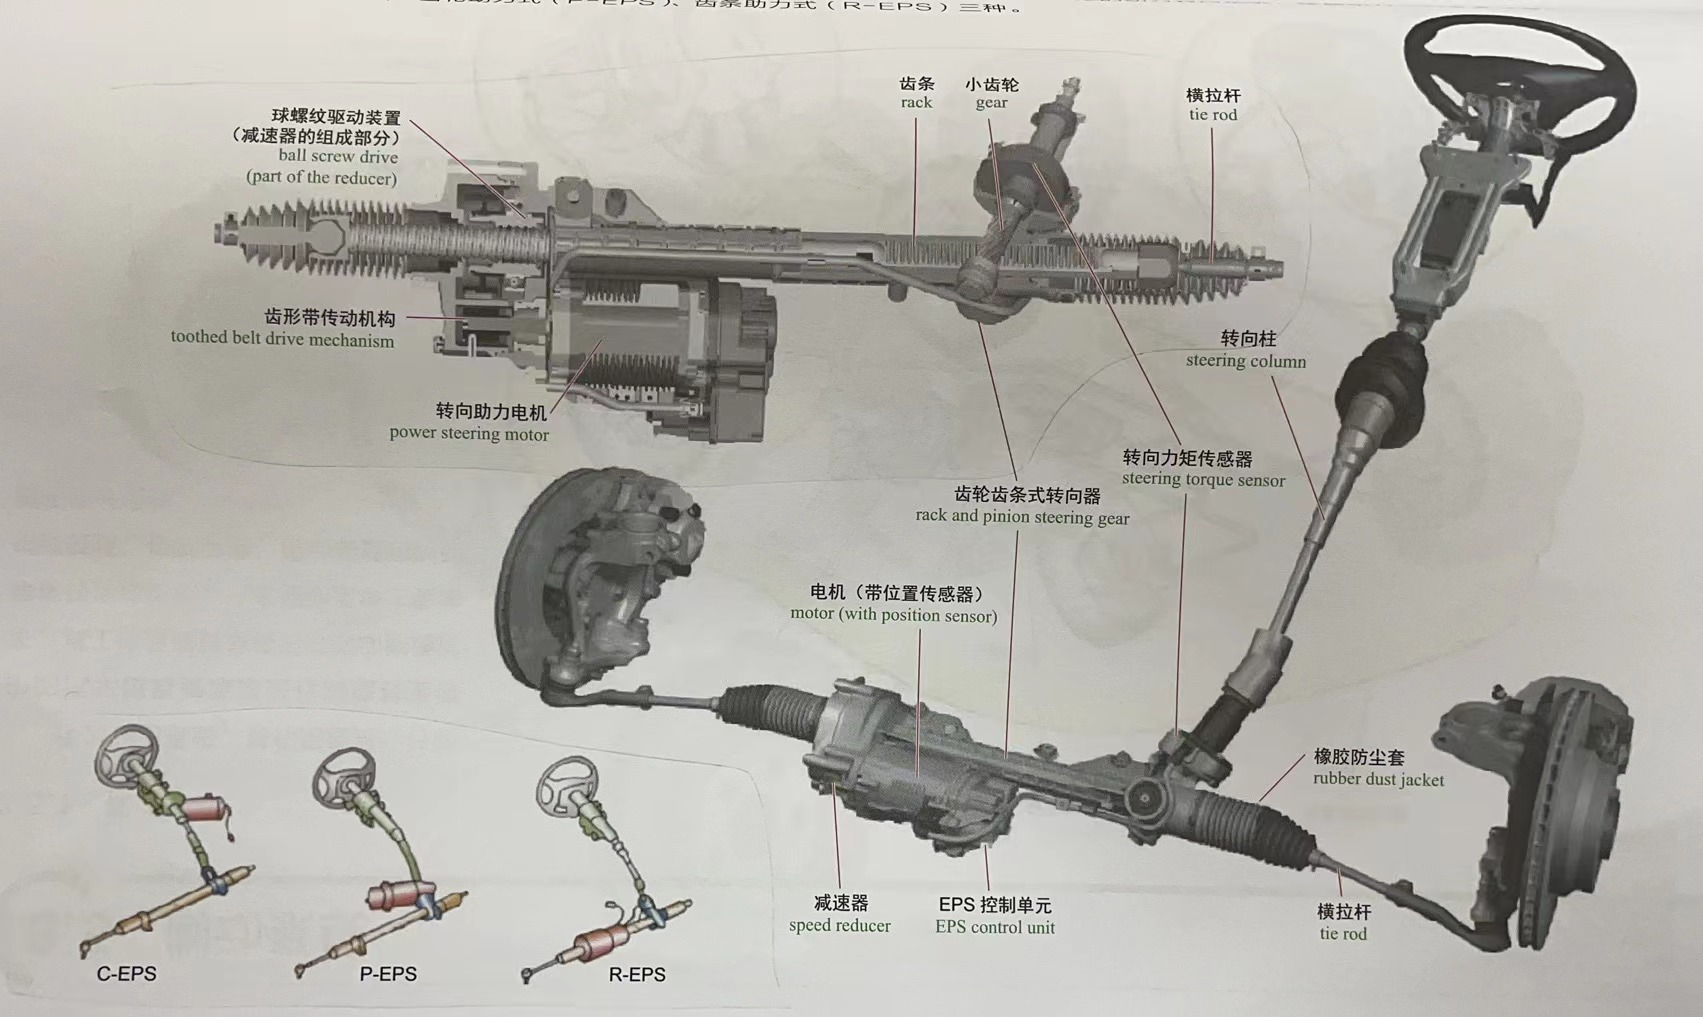
\includegraphics[width=0.5\textwidth]{3-38}
	\end{figure}
\section{制动系统}
\subsection{液压制动系统}
	\begin{center}
		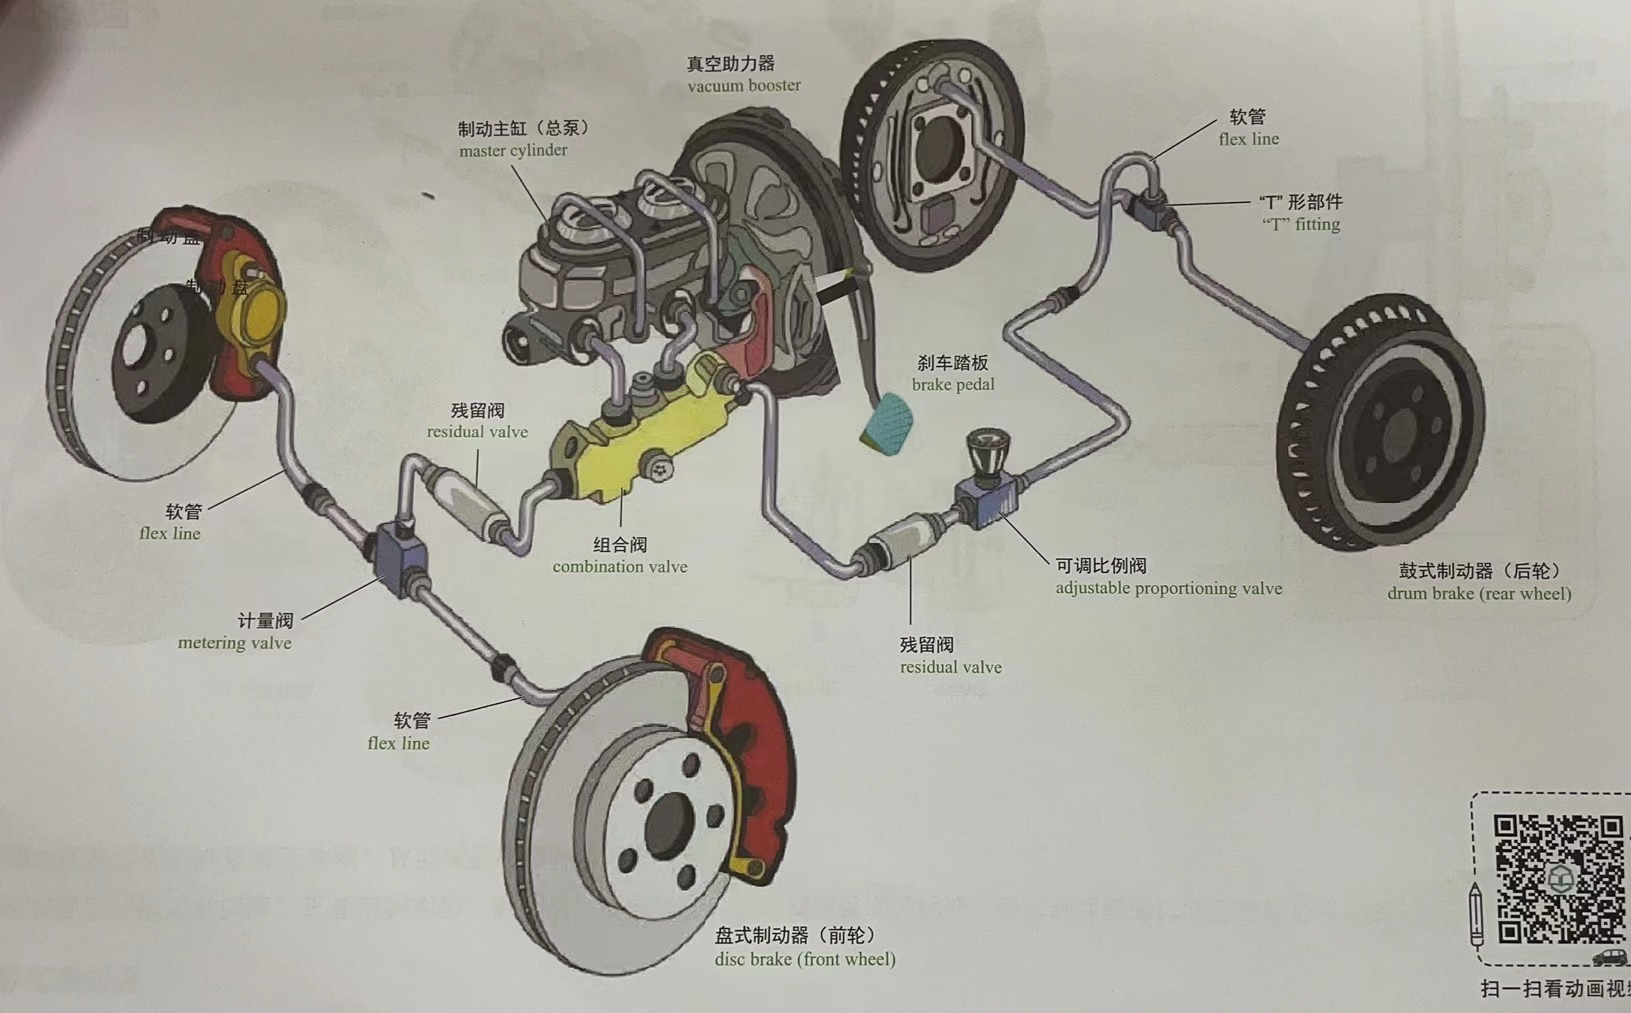
\includegraphics[width=0.5\textwidth]{3-39}
	\end{center}

\subsection{制动器}
	\subsubsection{盘式制动器}
		包括:制动盘、制动钳、摩擦片、分泵、油管
		
		液压油推动活塞,活塞拖动制动摩擦片,摩擦片压紧制动盘
		
		\begin{figure}[htbp]
			\centering
			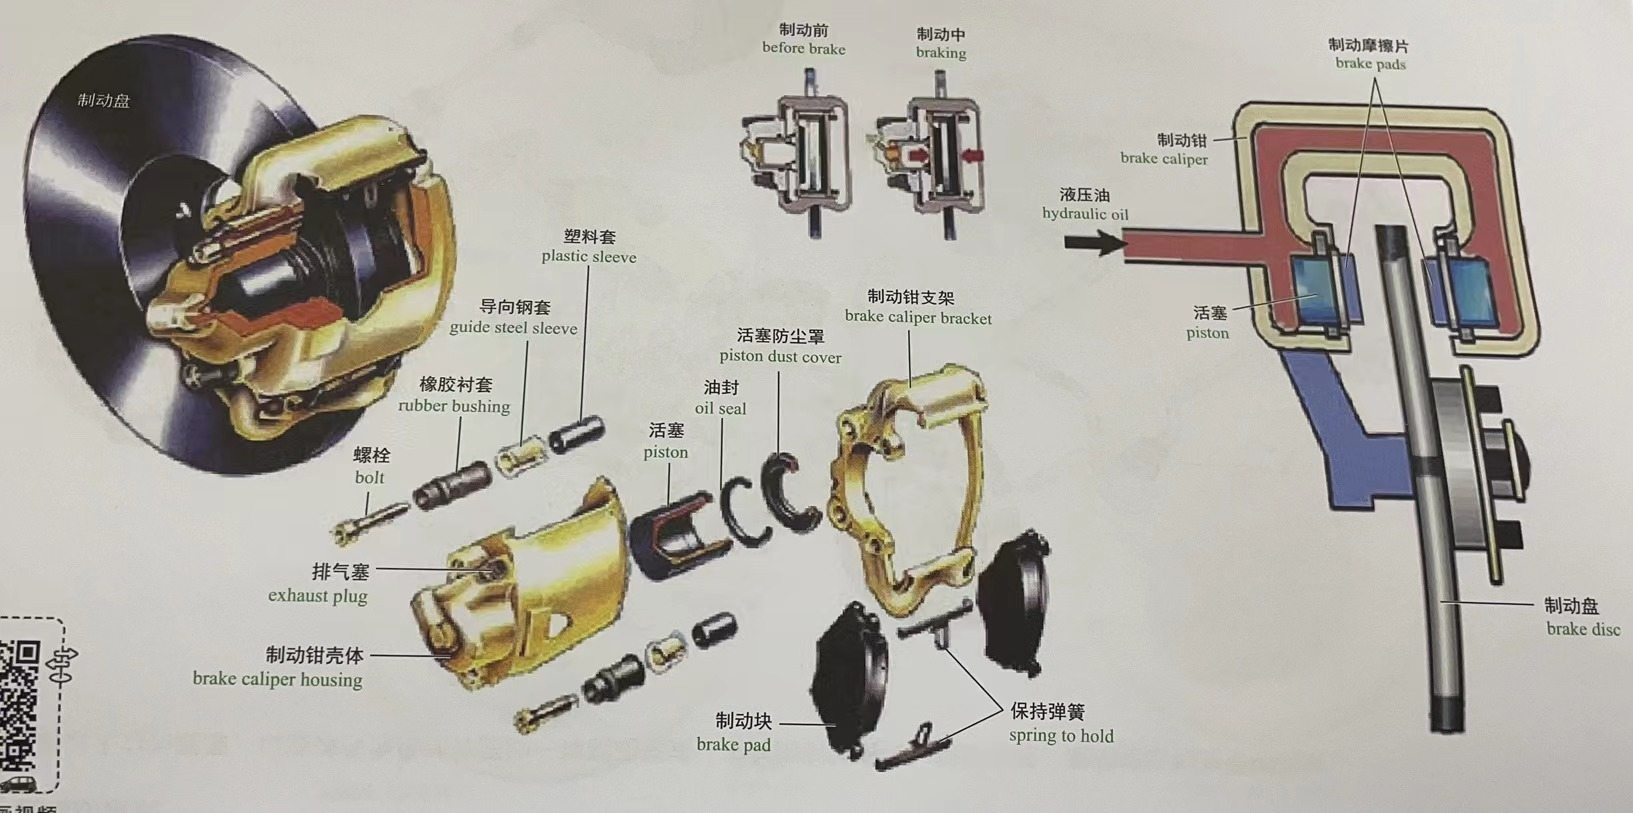
\includegraphics[width=0.5\textwidth]{3-40}
		\end{figure}
	\subsubsection{鼓式制动器}
		包括:制动轮缸、制动蹄、制动鼓、摩擦衬片、回位弹簧
		
		液压油往外推制动蹄,制动蹄往外推摩擦衬片,摩擦衬片压住制动鼓内侧
		\clearpage
\subsection{制动助力器}
	现在的汽车一般采用真空助力伺服制动系统(液压制动系统以外的一种制动系统)。
	
	传统燃油车的制动助力器为真空器助力器(下图黑色部分)。电动车的制动助力器为电动真空泵
	
	\begin{figure}[htbp]
		\centering
		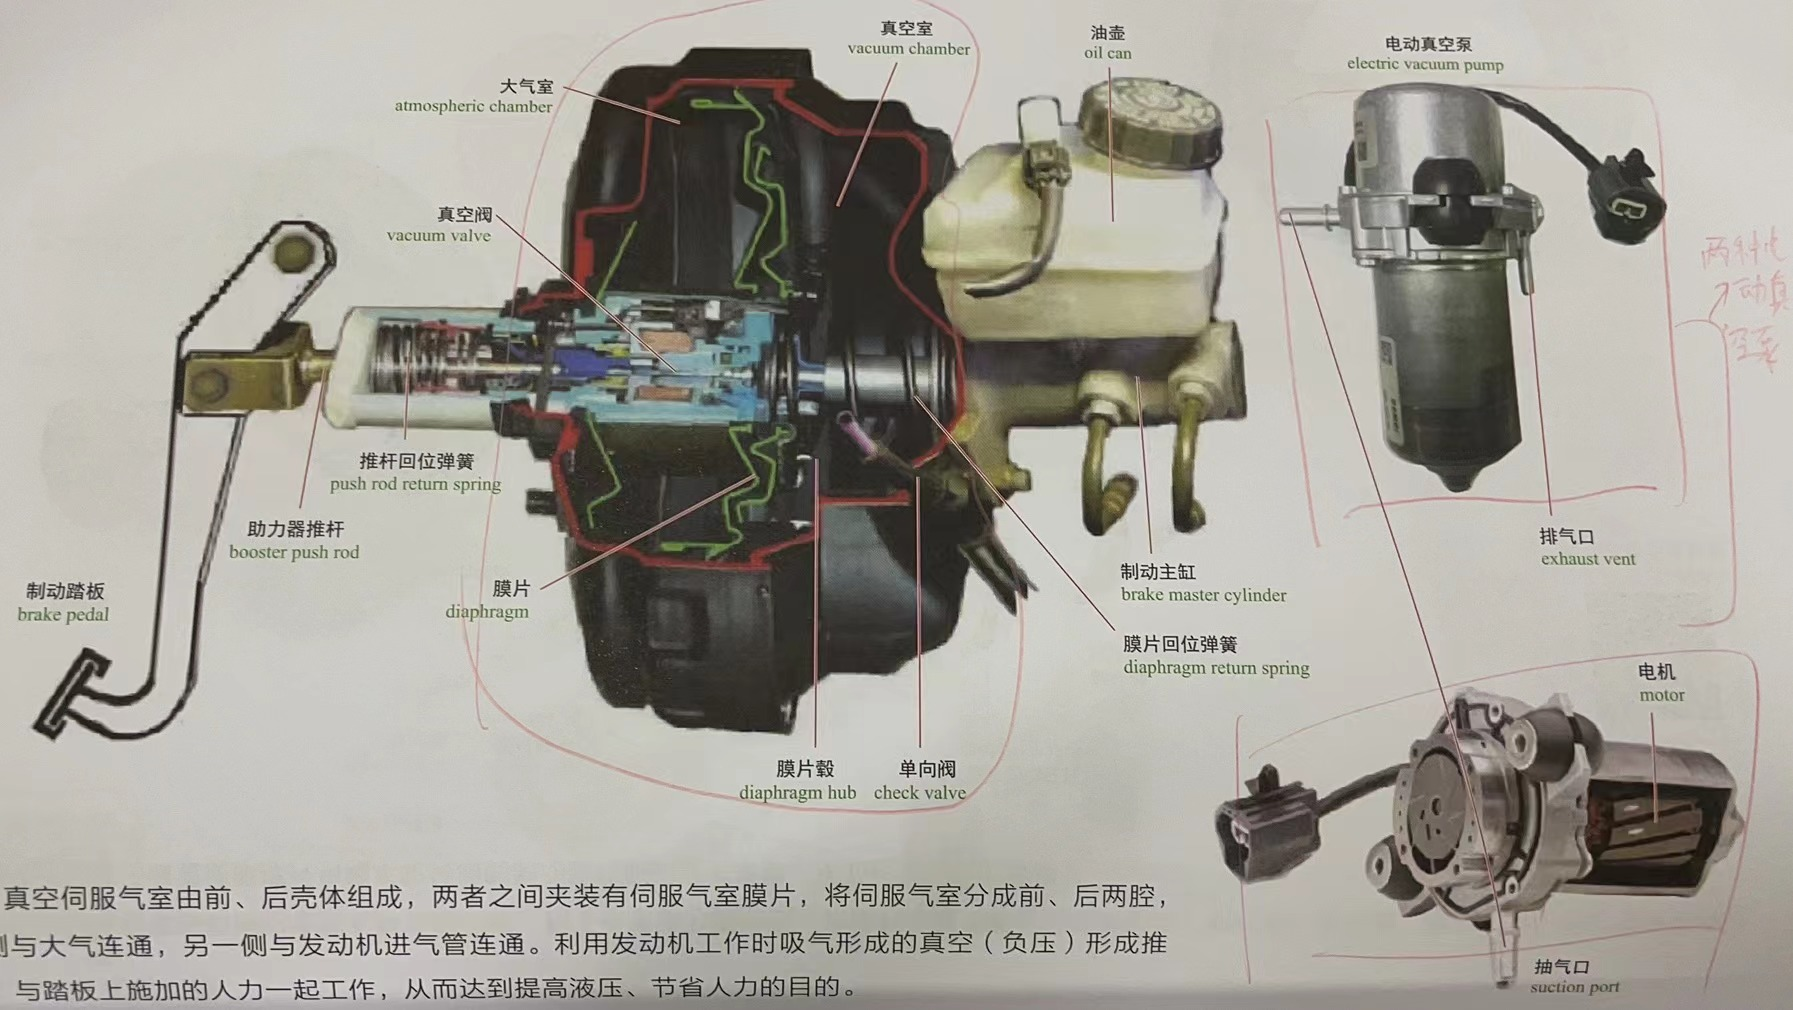
\includegraphics[width=0.5\textwidth]{3-41}
	\end{figure}
	
	真空助力器原理:发动机吸气时真空室气压减小,大气室气压大于真空室气压,形成一个大气室指向真空室的真空助力
\subsection{驻车制动器}
	包括制动器和驻车制动器拉杆(手刹)
	
	\begin{figure}[htbp]
		\centering
		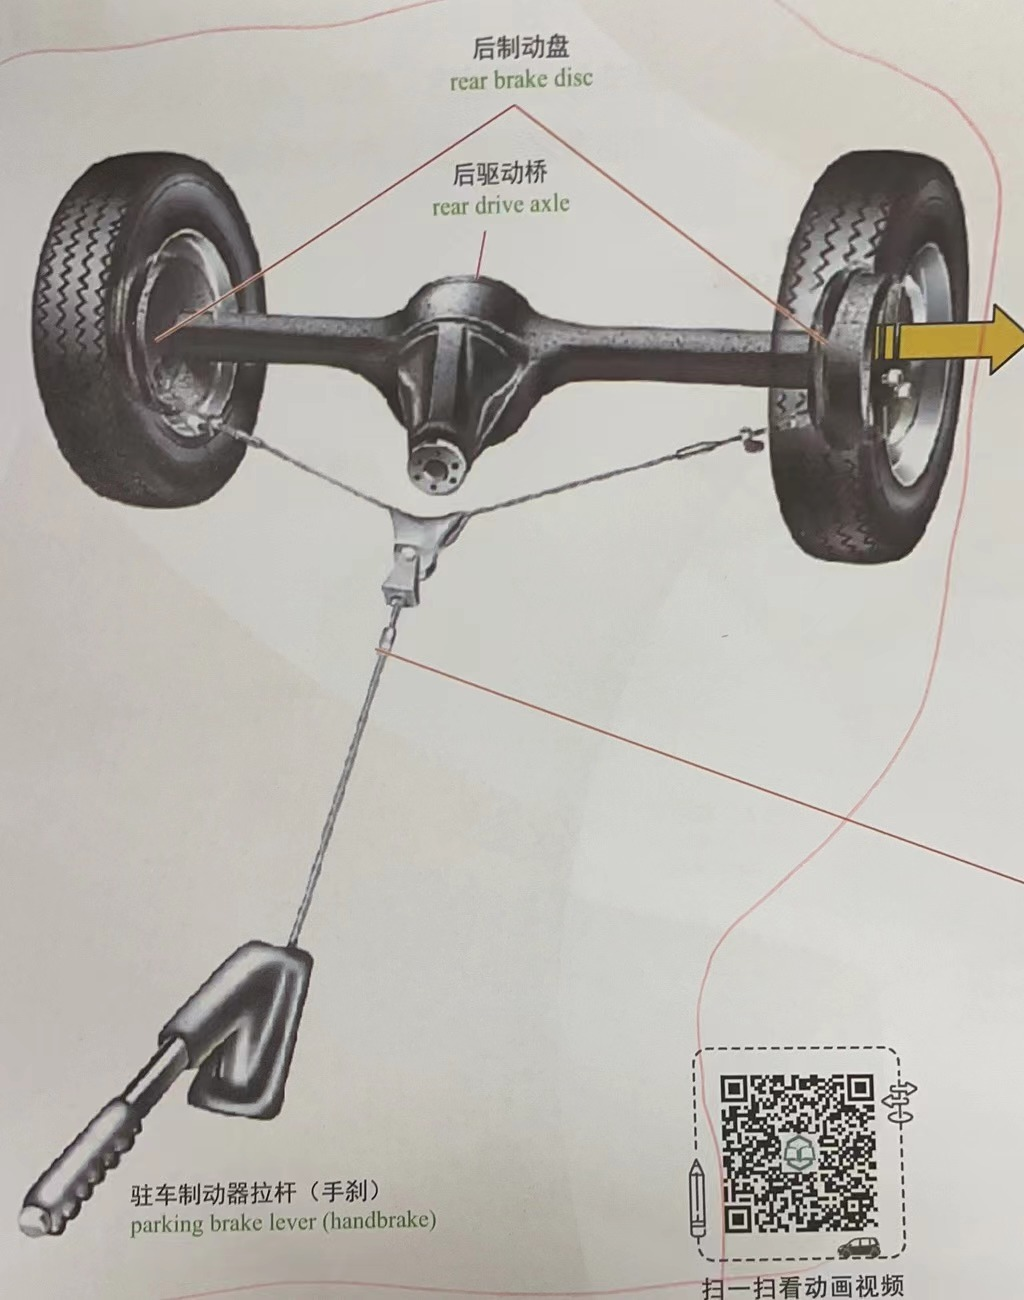
\includegraphics[width=0.5\textwidth]{3-42}
	\end{figure}
\end{document}